\appendix
\section*{附录}

\section{Overview}
% \begin{itemize}
%     \item \todo{Experiment.} compare pointnet with volumetric cnn and multi-view cnn on corrupted data (missing data). On both classification and segmentation. 
%     \item \todo{Writing.} network details.
%     \item \todo{Dump results.} more applications: normal prediction, correspondence, CAD model retrieval
%     \item (DONE) analysis on bottleneck and number of input points
%     \item (DONE) MNIST
%     \item \todo{Writing. Experiment.} details on object detection system
%     \item \todo{Dump results.} more output visualizations for critical points!! visualization of classification and part segmentation errors. visualization of detection results.
%     \item (DONE) proof of theorems
% \end{itemize}
该文件为主要论文提供了额外的定量结果,技术细节和更多定性的测试示例。 

在 Sec~\ref{sec:cla_robust}中,我们扩展了健壮性测试,以比较不完整输入下的PointNet和VoxNet。 在 Sec~\ref{sec:network}中我们提供了更多有关神经网络架构和训练参数的详细信息, 在 Sec~\ref{sec:detection}中我们描述了场景中的检测流程。Sec~\ref{sec:supp_application} 显示了PointNet的更多应用, 而 Sec~\ref{sec:architecture} 显示了更多的分析实验。 Sec~\ref{sec:proof} 为我们在PointNet上的理论提供了证明。 最后,我们在 Sec~\ref{sec:visu}中显示了更多的可视化结果。


\section{PointNet和VoxNet的比较 (Sec 5.2)}
\label{sec:cla_robust}
我们扩展了第 5.2 节鲁棒性测试中的实验,以比较PointNet和VoxNet~\cite{maturana2015voxnet}(一个用于体积表示的代表性结构)对输入点云中缺失数据的鲁棒性。两个网络都在以 1024 个点作为输入的相同训练测试集上进行训练。对于VoxNet,我们将点云体素化为 $32 \times 32 \times 32$ 的网格,并通过绕上轴随机旋转和抖动来增加训练数据。

在测试时,输入点按一定比例随机丢弃。由于VoxNet对旋转很敏感,它的预测使用来自点云的 12 个视点的平均分数。如图~\ref{fig:compare}所示,我们的PointNet对缺失点更加鲁棒。 当一半的输入点丢失时,VoxNet 的准确率急剧下降,从 $86.3\%$ 到 $46.0\%$,相差 $40.3\%$,而我们的 PointNet 的性能下降只有 $3.7\%$。这可以通过我们 PointNet 的理论分析和解释来解释——它正在学习使用 \textit{critical points} 的集合来总结形状,因此它对缺失数据非常健壮。


\begin{figure}[h!]
    \centering
    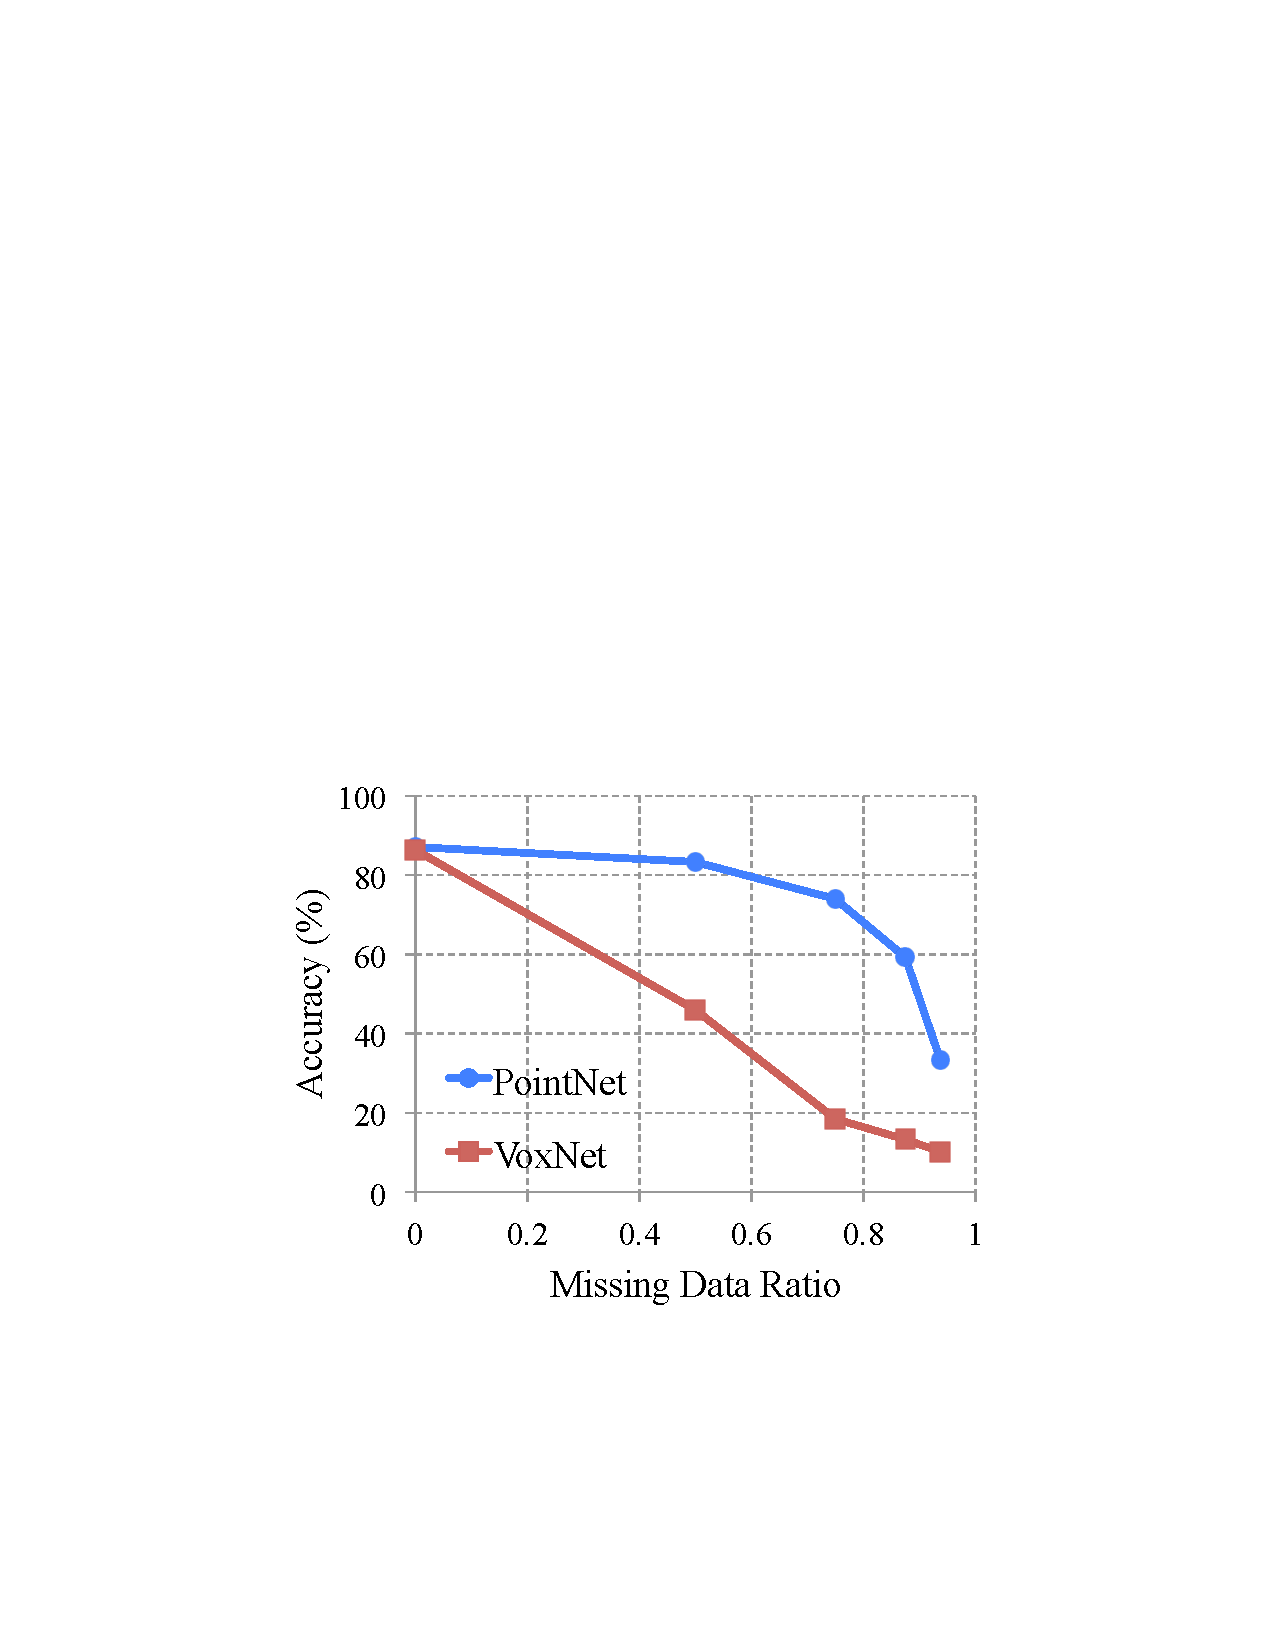
\includegraphics[width=0.7\linewidth]{fig/pointnet_vs_voxnet.pdf}
    \caption{\textbf{在不完整输入数据下的PointNet v.s. VoxNet~\cite{maturana2015voxnet} } 指标是 ModelNet40 测试集上的整体分类准确率。请注意,VoxNet 使用 12 个视点平均,而 PointNet 仅使用点云的一个视图。显然 PointNet 对缺失点具有更强的鲁棒性。}
    \label{fig:compare}
\end{figure}

% =============================
% Network details
% =============================
\section{网络架构和训练细节 (Sec 5.1)}
\label{sec:network}
\paragraph{PointNet分类网络}由于论文正文中已经说明了基本的体系结构,因此我们在此处提供有关联合对齐/变换网络和训练参数的更多详细信息。

第一个转换网络是一个mini-PointNet,它直接以未处理的点云为输入,并回归成一个$3\times3$的矩阵。这个网络由一个每个点共享的 $MLP(64,128,1024)$ 网络(输出尺寸分别为64, 128, 1024), 一个点间max pooling和两个全连接层(输出尺寸分别为$512$, $256$)组成。输出矩阵初始值为单位矩阵。除了最后一层,其余所有层都应用了ReLU和Batch Normalization。 第二个变换网络与第一个结构相同,除了输出矩阵尺寸为$64\times64$。输出矩阵也被初始化为单位阵。将正则化损失(权重为0.001)添加到softmax分类损失中,以使矩阵接近正交。

训练时,在估计类别概率前,对最后一层全连接层(维度$256$)应用了keep ratio 为$0.7$的dropout。
Batch Normalization的衰减率从初始的$0.5$逐渐增加到$0.99$。使用adam优化器,初始学习率设置为$0.001$,momentum为$0.9$,batch size为$32$。学习率每迭代20次下降一半。在TensorFlow下用GTX1080 GPU和ModelNet数据集训练,网络需要3-6个小时收敛。

\paragraph{PointNet分割网络}分割网络是PointNet分类网络的一个延伸。对于每个点,将局部点特征(第二个转换网络之后的输出)和全局特征(max pooling的输出)连接在一起。 在分割网络中不使用dropout。训练参数与分类网络相同。

关于形状零件分割的任务,我们对基本分割网络体系结构进行了一些修改 (正文中的图2) 以实现最佳性能。如图~\ref{fig:part_seg_net}所示。 我们添加了一个one-hot向量来显示输入类别并与max pooling的输出连接。 我们还在某些层中增加了神经元个数,并添加了skip links以收集不同层中的局部点特征,并将它们连接起来以形成点特征输入到分割网络中。

\begin{figure}
\centering
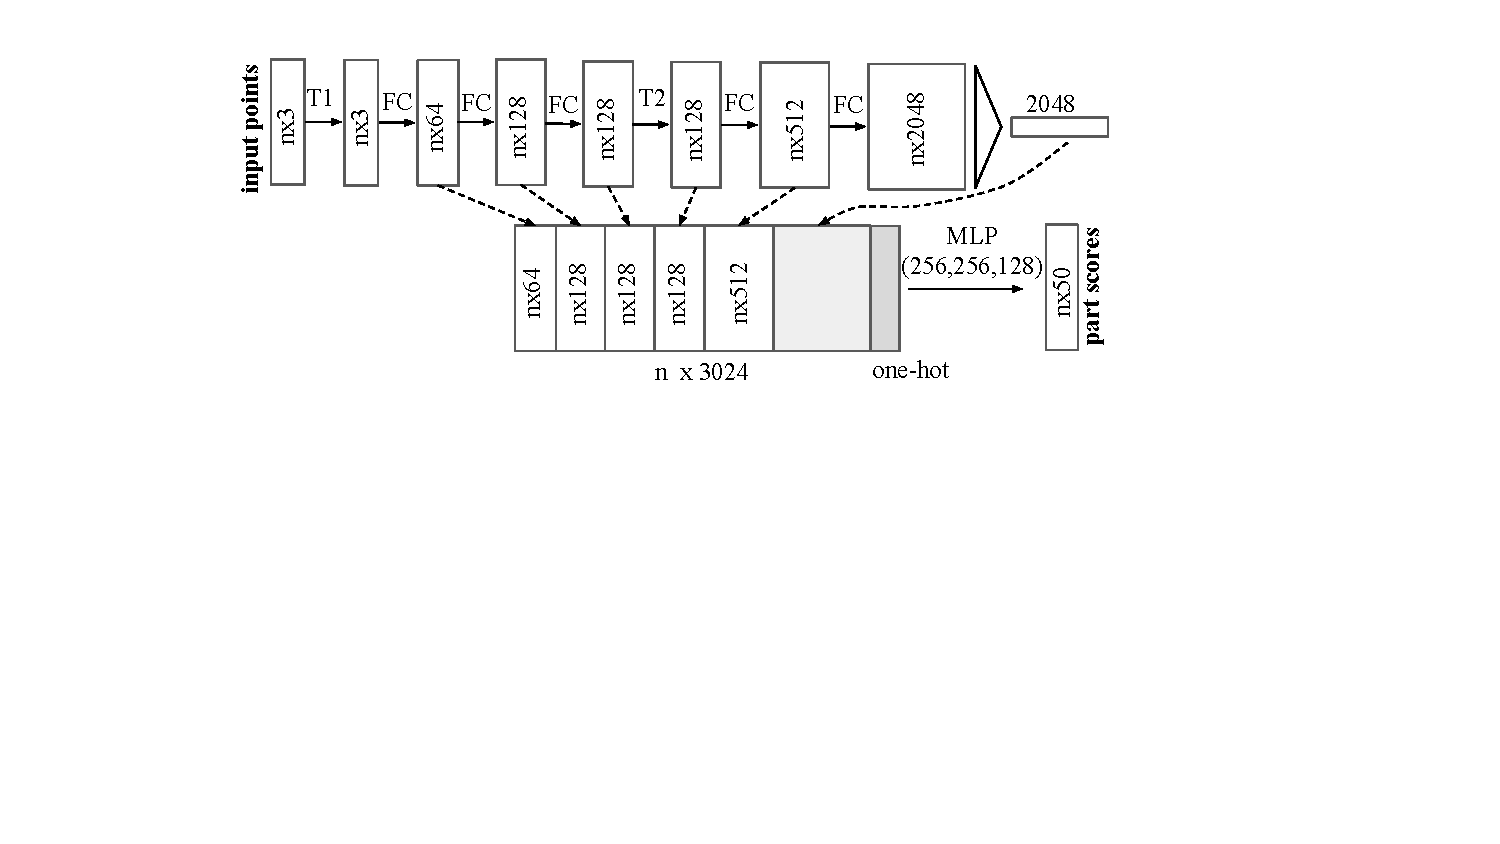
\includegraphics[width=\linewidth]{fig/part_seg_net.pdf}
\caption{\textbf{零件分割的网络架构} T1和T2是输入点和特征的对齐/变换网络。FC是在每个点上操作的全连接层。MLP是每一点上的多层感知器。One-hot是一个大小为16的向量,表示输入形状的类别。}
\label{fig:part_seg_net}
\end{figure}

尽管 \cite{Wu2014248} 和 \cite{Yi16} ]独立地处理每个对象类别, 但由于缺少某些类别的训练数据 (第一行显示了数据集中所有类别的形状总数), 我们训练了跨类别的PointNet(但是使用one-hot向量来指示类别).为了进行公平比较,在测试这两个模型时,我们只预测给定特定对象类别的部分标签。

对于语义学分割任务,应用的是与论文主体中相同的基本网络结构,如图2。

使用ShapeNet part 数据集训练需要大约6-12小时,使用Stanford semantic parsing数据集训练大概需要半天。

\paragraph{基准3D CNN分割网络}
在ShapeNet零件分割实验中,我们将建议的分割版本PointNet与两种传统方法以及3D体积CNN网络基准进行了比较。 在图~\ref{fig:voxnet}中, 我们展示了我们使用的基准3D体积CNN网络。 我们将众所周知的3D CNN架构,例如VoxNet \cite{maturana2015voxnet} 和 3DShapeNets \cite{wu20153d} 推广到完全卷积的3D CNN分割网络。

%In the CAD model part segmentation experiment, we compare our proposed segmentation version PointNet to two traditional methods based on shape local features and inter-shape correspondence, as well as a 3D volumetric CNN network as baseline methods. Our PointNet method is a data-driven deep learning method. The comparison between traditional methods to data-driven methods are inherently hard since data-driven methods require more training data than traditional methods. Though we try to test all the methods on the same ShapeNet train/validation/test split, we still think it is crucial to compare our proposed learning-based PointNet with another deep learning method. In Fig.~\ref{fig:voxnet}, we show the baseline 3D volumetric CNN network we use. We generalize the well-known 3D CNN architectures, such as VoxNet \cite{maturana2015voxnet} and 3D ShapeNet \cite{wu20153d} that are invented for classification task, to a 3D CNN segmentation network.

\begin{figure}[t!]
\centering
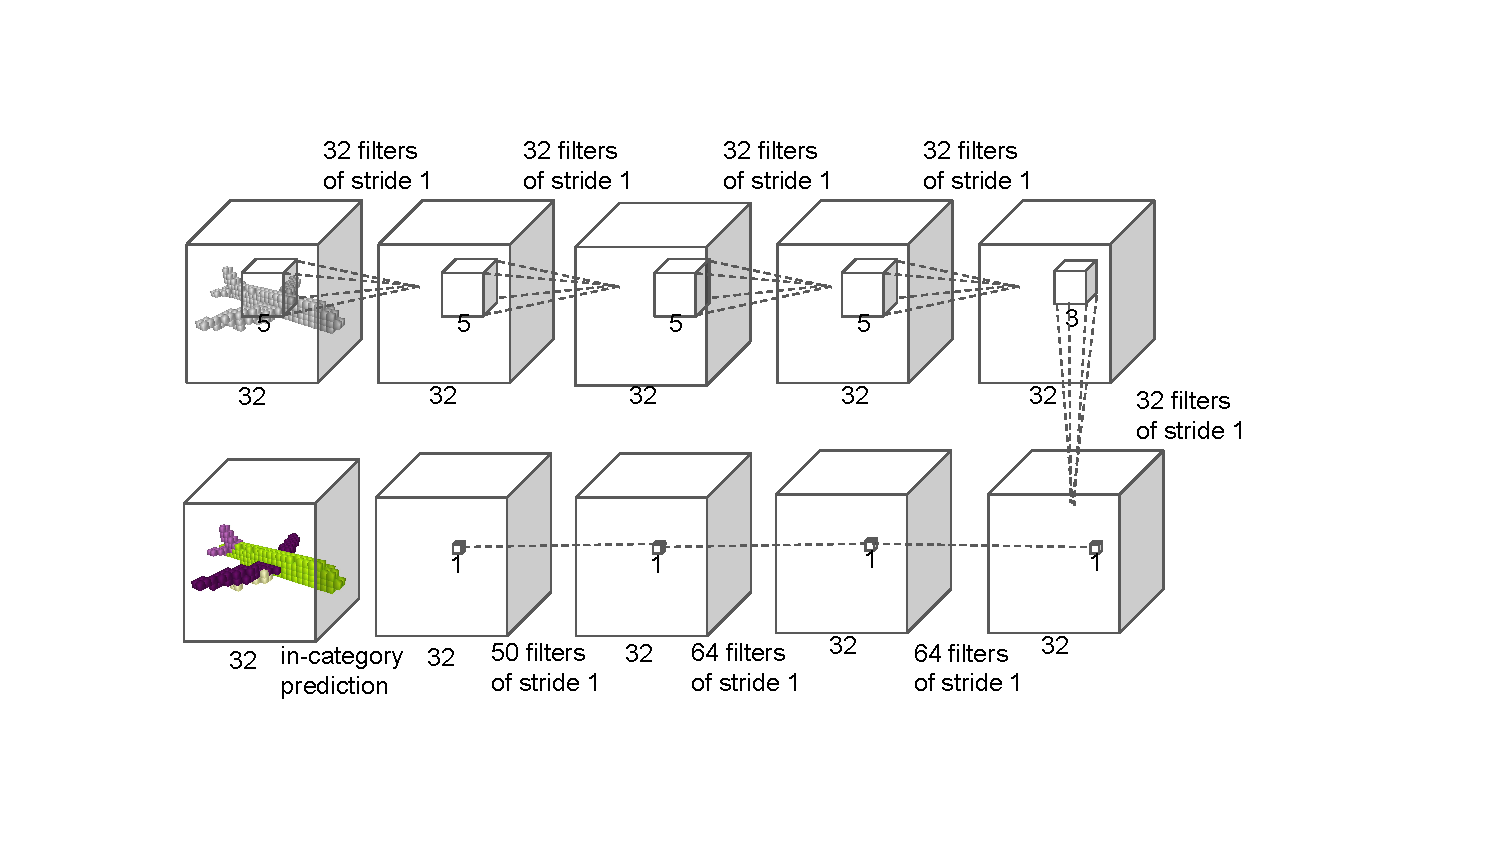
\includegraphics[width=\linewidth]{fig/voxnet.pdf}
\caption{\textbf{基准3D CNN分割网络.} 该网络是完全卷积化的,并且可以预测每个体素的部分分数}
\label{fig:voxnet}
\end{figure}
对于给定的点云,我们首先将其转换为具有$32 \times 32 \times 32$分辨率的占用网格的体积表示形式。然后,依次使用五个具有32个输出通道和步长为1的3D卷积核来提取特征。每个体素的感受野为19。 %In order to do the final per-pixel label prediction, we choose to keep the size of the feature maps to $32 \times 32 \times 32$ by allowing zero-padding. Zero-padding is reasonable since there are no occupancy for those padded voxels.
最后,将大小为$1\times 1\times 1$的3D卷积序列附加到计算出的特征图上,以预测每个体素的分割标签。除最后一层外,所有层均使用ReLU和Batch Normalization。该网络是跨类别训练的,但是,为了与给出对象类别的其他基准方法进行比较,我们仅考虑给定对象类别中的输出得分。

\section{Details on Detection Pipeline (Sec 5.1)}
\label{sec:detection}
我们基于语义分割结果和我们的对象分类 PointNet 构建了一个简单的 3D 对象检测系统。

我们使用带有分割分数的连接组件来获取场景中的对象提议。从场景中的一个随机点开始,我们找到它的预测标签,并使用 BFS 搜索附近具有相同标签的点,搜索半径为 $0.2$ 米。如果结果集群有超过 200 个点(假设 1m x 1m 区域中有 4096 个点样本),则集群的边界框被标记为一个对象提议。对于每个提议的对象,它的检测分数计算为该类别的平均点分数。在评估之前,面积/体积极小的提案被裁剪。对于桌子、椅子和沙发,边界框会延伸到地板,以防腿与座椅/表面分开。

我们观察到,在某些房间(例如礼堂)中,许多物体(例如椅子)彼此靠近,其中连接的组件无法正确地分割出单个的物体。因此,我们利用我们的分类网络并使用滑动形状方法来缓解椅子类的问题。我们为每个类别训练一个二元分类网络,并使用分类器进行滑动窗口检测。结果框通过非最大抑制进行裁剪。将来自连接组件和滑动形状的建议框组合起来进行最终评估。

在 图~\ref{fig:pr_curve} 中,我们展示了目标检测的准确率-召回率曲线。 我们训练了六个模型,其中每个模型都在五个区域进行训练并在左侧区域进行测试。在测试阶段,每个模型都在它从未见过的区域进行测试。将所有六个区域的测试结果汇总以生成 PR 曲线。
 
 \begin{figure}
 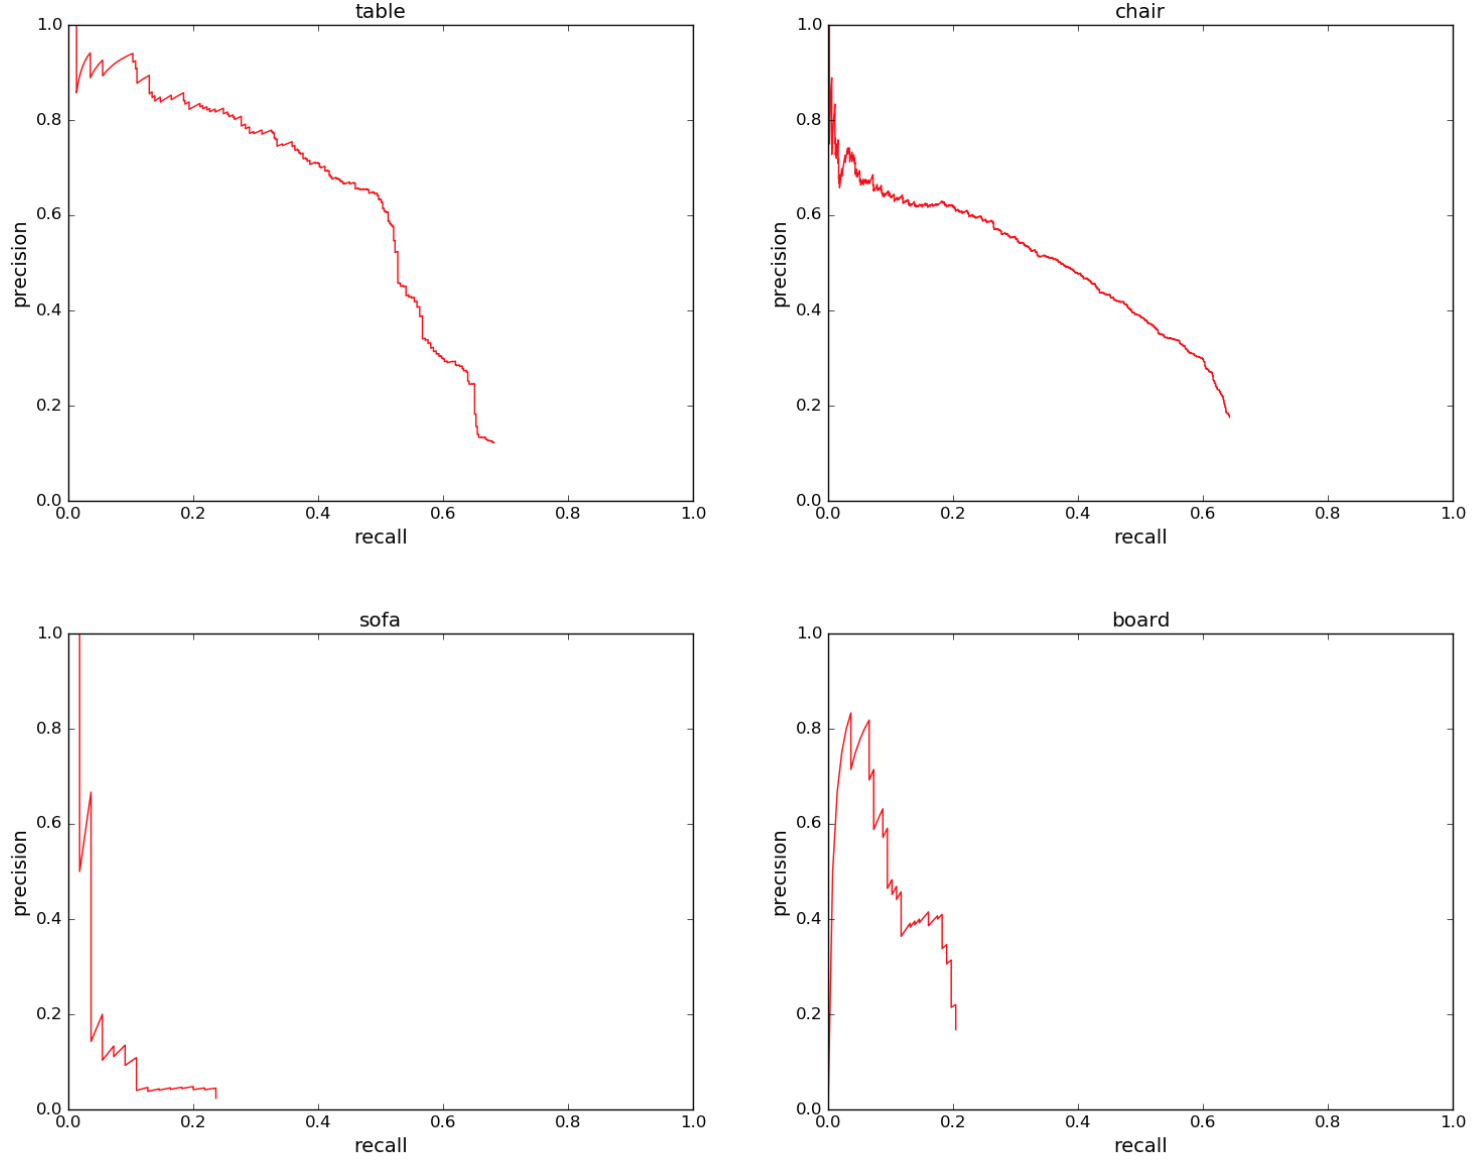
\includegraphics[width=0.8\linewidth]{fig/pr_curve.png}
 \centering
 \caption{\textbf{用于 3D 点云中对象检测的准确率-召回率曲线。} 我们在所有的六个区域上对四个类别进行了评估:桌子、椅子、沙发和木板。 IoU 阈值在体积上表现为 0.5 。}
 \label{fig:pr_curve}
 \end{figure}
 
% =============================
% More Applications
% =============================
\section{更多应用 (Sec 5.1)}
\label{sec:supp_application}
\paragraph{从点云中检索模型} 我们的 PointNet 为每个给定的输入点云学习全局形状特征。我们期望几何相似的形状具有相似的全局特征。在本节中,我们将在形状检索应用程序上测试我们的猜想。更具体地说,对于由 ModelNet 划分的测试集中每个给定查询形状,我们计算其由我们的分类 PointNet 给出的全局签名(分数预测层之前的层的输出),并通过最近邻搜索在划分的训练集中检索相似的形状。结果如图~\ref{fig:retrieval}所示。

\begin{figure}[h]
    \centering
    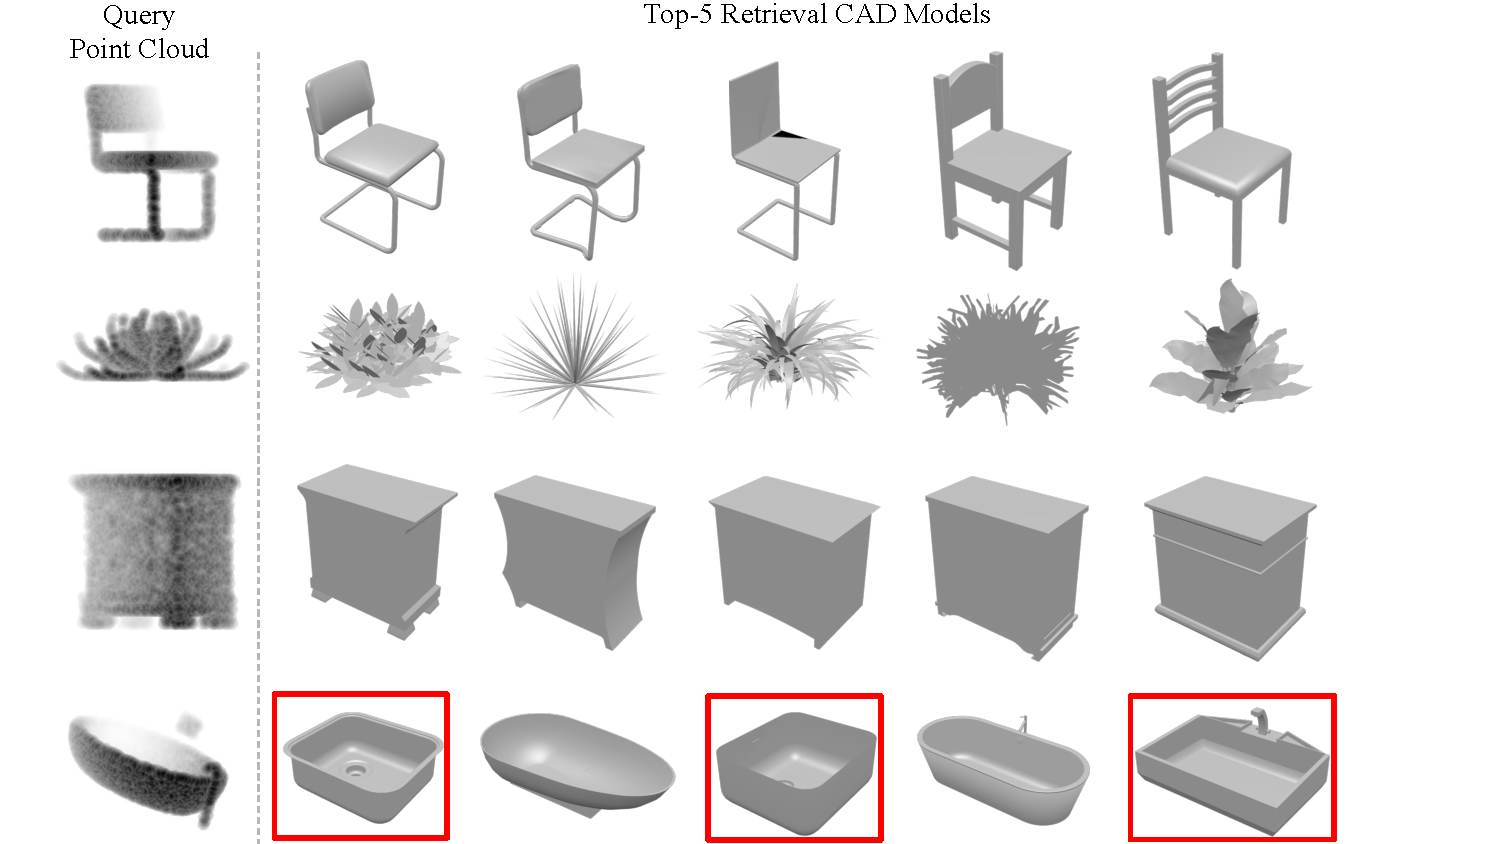
\includegraphics[width=\linewidth]{fig/retrieval.pdf}
    \caption{\textbf{从点云中检索模型。} 对于每个给定的点云,我们从 ModelNet 划分的测试集中检索前 5 个相似的形状。 从上到下,我们展示了椅子、植物、床头柜和浴缸查询的示例。错误类别的检索结果用红色框标记。}
    \label{fig:retrieval}
\end{figure}

\paragraph{形状对应}
%Since our PointNet learns many per-point functions at the first stage and then aggregates the computed per-point features together using a max-pooling to compute the global shape feature. Thus, there is an inherent correspondence between every coordinate of the global features for a pair of shapes. 

在本节中,我们展示了 PointNet 学习的点特征可以潜在地用于计算形状对应。 给定两个形状,我们通过匹配激活全局特征中相同维度的点对来计算它们的 \textit{critical point sets} $C_S$ 之间的对应关系。Fig~\ref{fig:chair_corr} 和 Fig~\ref{fig:table_corr} 显示了检测到的两个相似椅子和桌子之间的形状对应关系。

\begin{figure}[h]
    \centering
    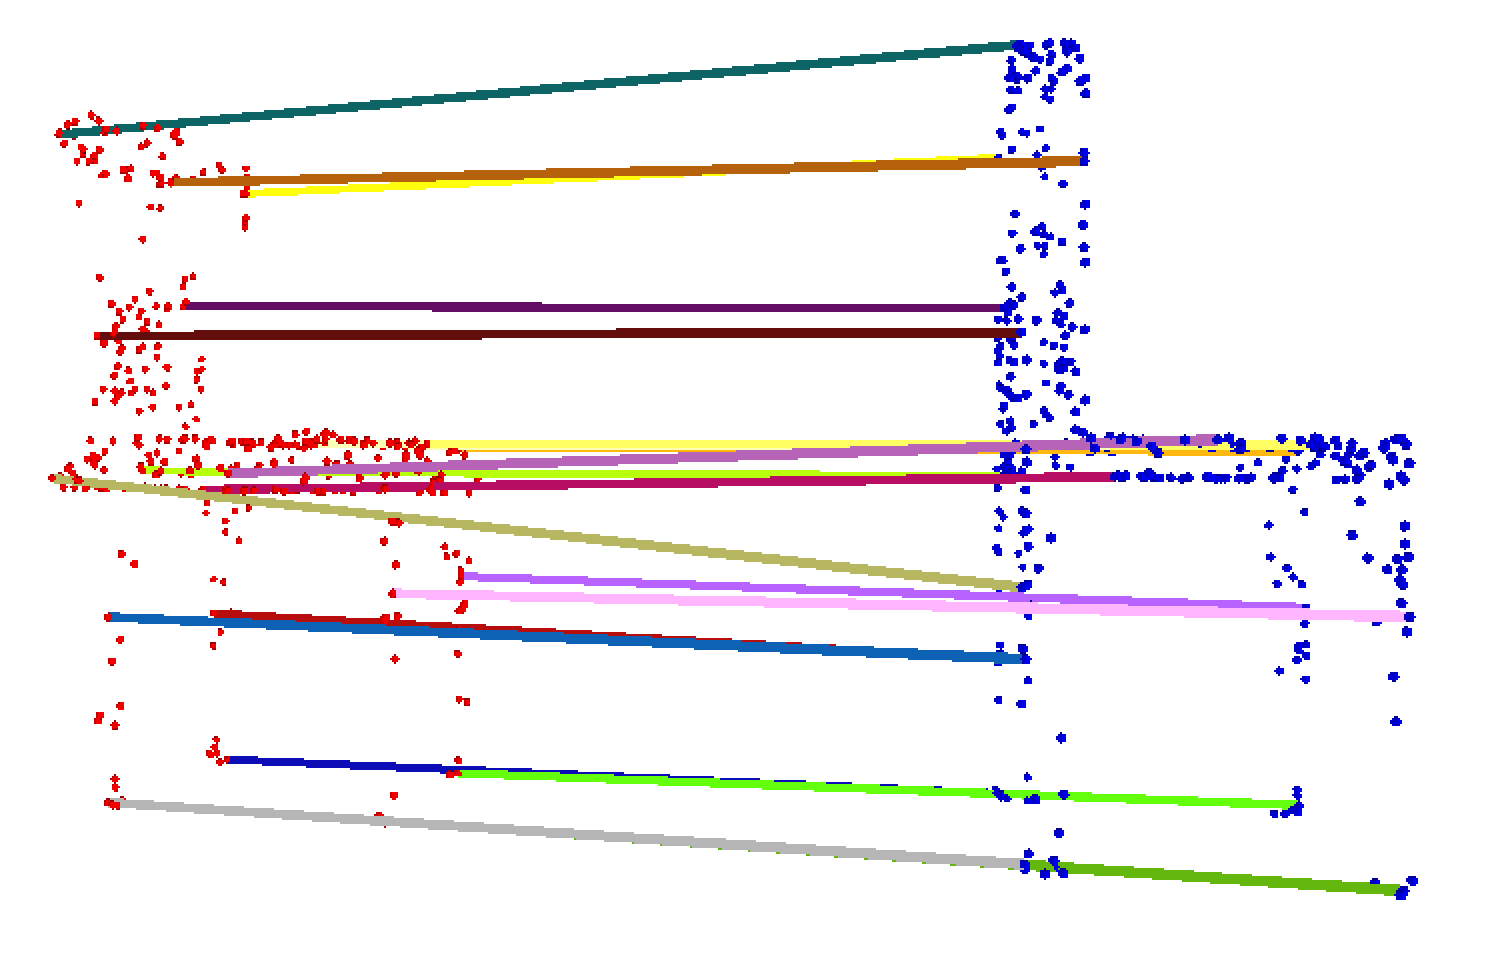
\includegraphics[width=\linewidth]{fig/chair_corr.png}
    \caption{\textbf{两个椅子之间的形状对应。} 为了可视化的清晰性,我们只展示了 20 个随机挑选的映射对。}
    \label{fig:chair_corr}
\end{figure}

\begin{figure}[h]
    \centering
    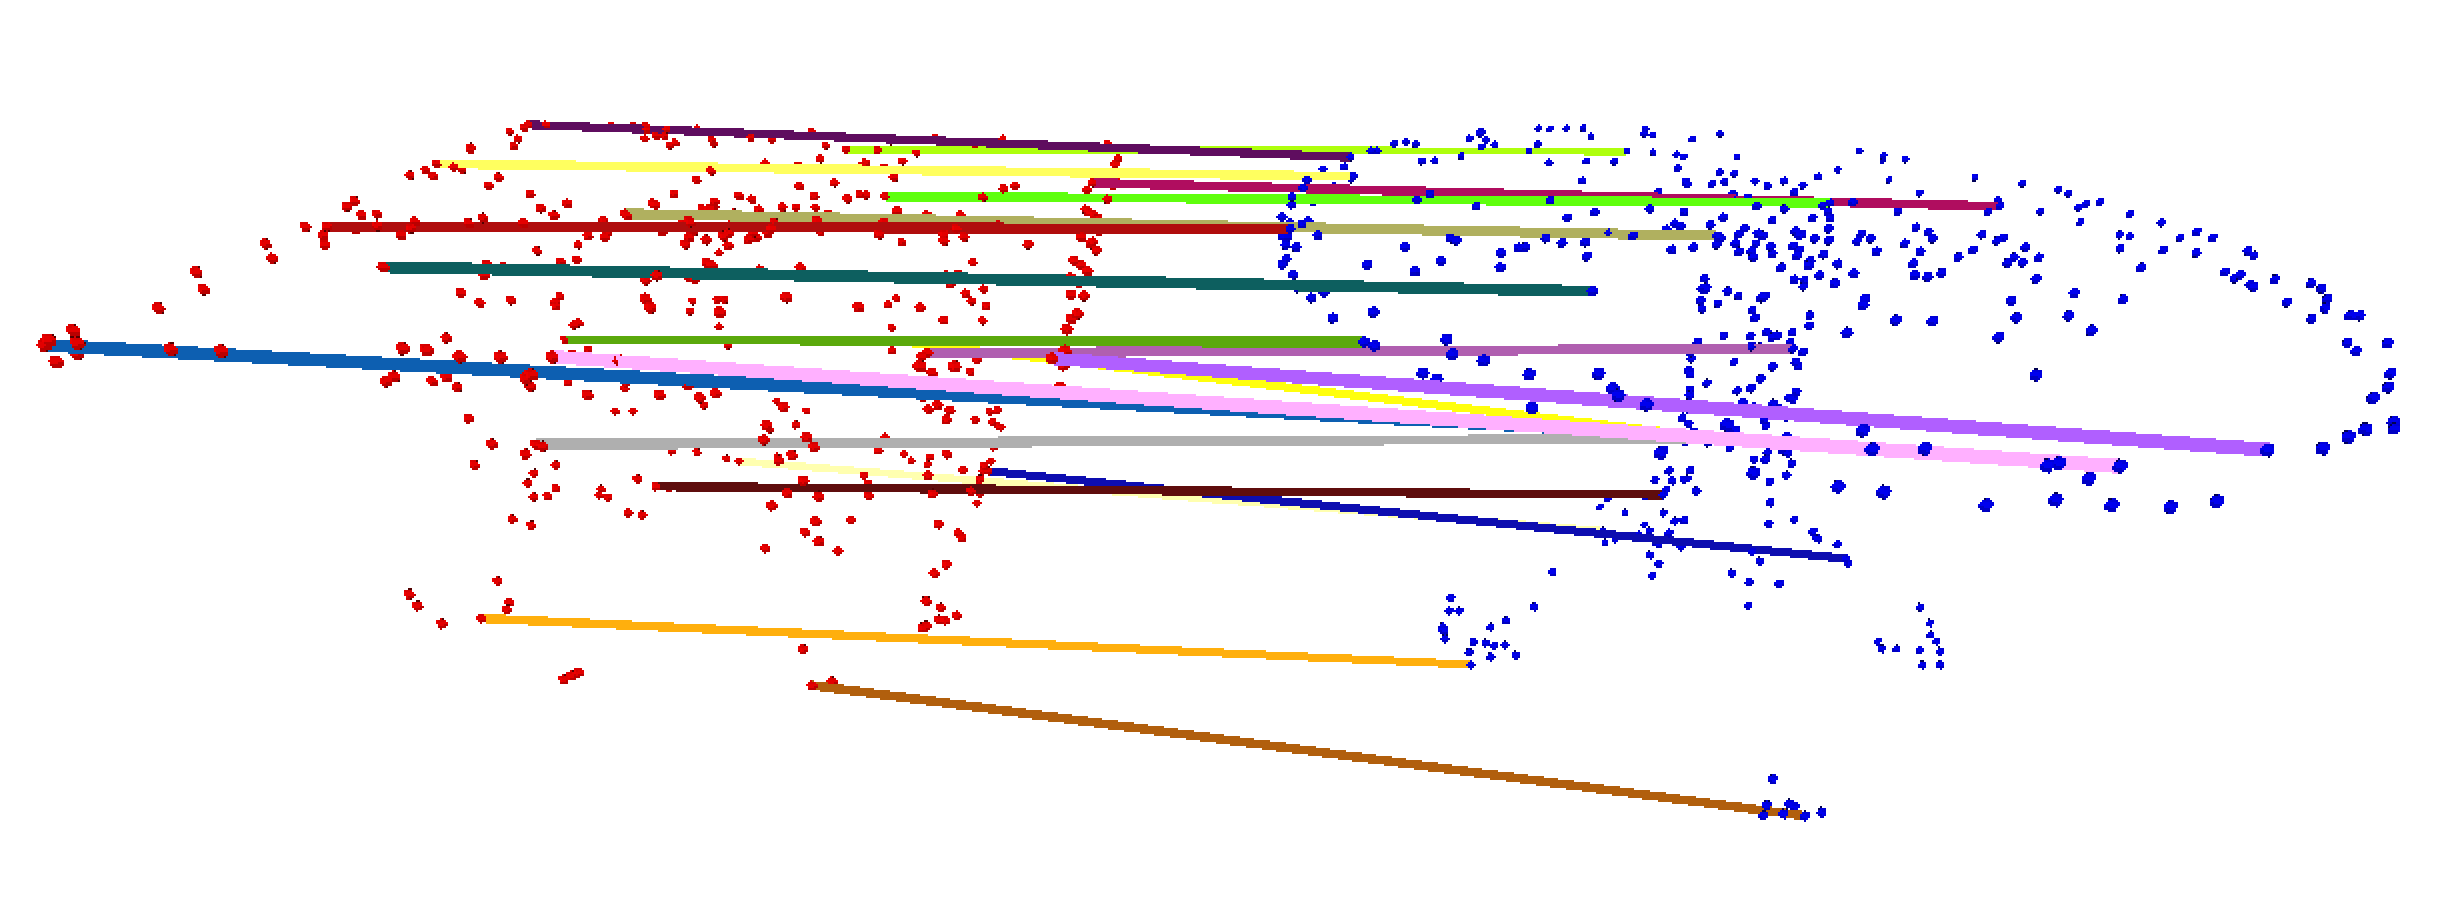
\includegraphics[width=\linewidth]{fig/table_corr.png}
    \caption{\textbf{两张桌子之间的形状对应。} 为了可视化的清晰性,我们只展示了 20 个随机挑选的映射对。}
    \label{fig:table_corr}
\end{figure}


% =============================
% More Architecture Analysis
% =============================
\section{更多结构分析 (Sec 5.2)}
\label{sec:architecture}
% \paragraph{Volumetric Reconstruction} To validate proof under Thm2 saying that in the worst case our network will degrade to learn a volumetric respentation for the 3D shape? 

\paragraph{瓶颈维度和输入点数量的有效性}

根据第一个输入层的大小和输入点云的数量,我们的模型的表现会有所变化,接下来我们将阐释其变化。 从图 ~\ref{fig:net_param} 中我们可以看出,随着我们提高点的数量,性能变得越来越好。在大约 1000 个点时,达到饱和。最大的层尺寸同样起了重要作用,让我们将层大小从 64 增大到 1024 之后,表现提升了 $2-4\%$。这说明我们需要足够多的,覆盖整个三维空间的点特征函数来分辨不同的形状。



% \paragraph{Effects of Bottleneck Dimension and Number of Input Points}
% Here we show our model's performance change with regard to the size of the first max layer output as well as the number of input points. In Fig~\ref{fig:net_param} we see that performance grows as we increase the number of points however it saturates at around 1K points. The max layer size plays an important role, increasing the layer size from 64 to 1024 results in a $2-4\%$ performance gain. It indicates that we need enough point feature functions to cover the 3D space in order to discriminate different shapes.

值得一提的是,即便有 64 个点作为了输入(从网络上采样的点中最远的点),我们的网络仍然能够取得令人满意的效果。

% It's worth notice that even with 64 points as input (obtained from furthest point sampling on meshes), our network can achieve decent performance.

\begin{figure}[h]
    \centering
    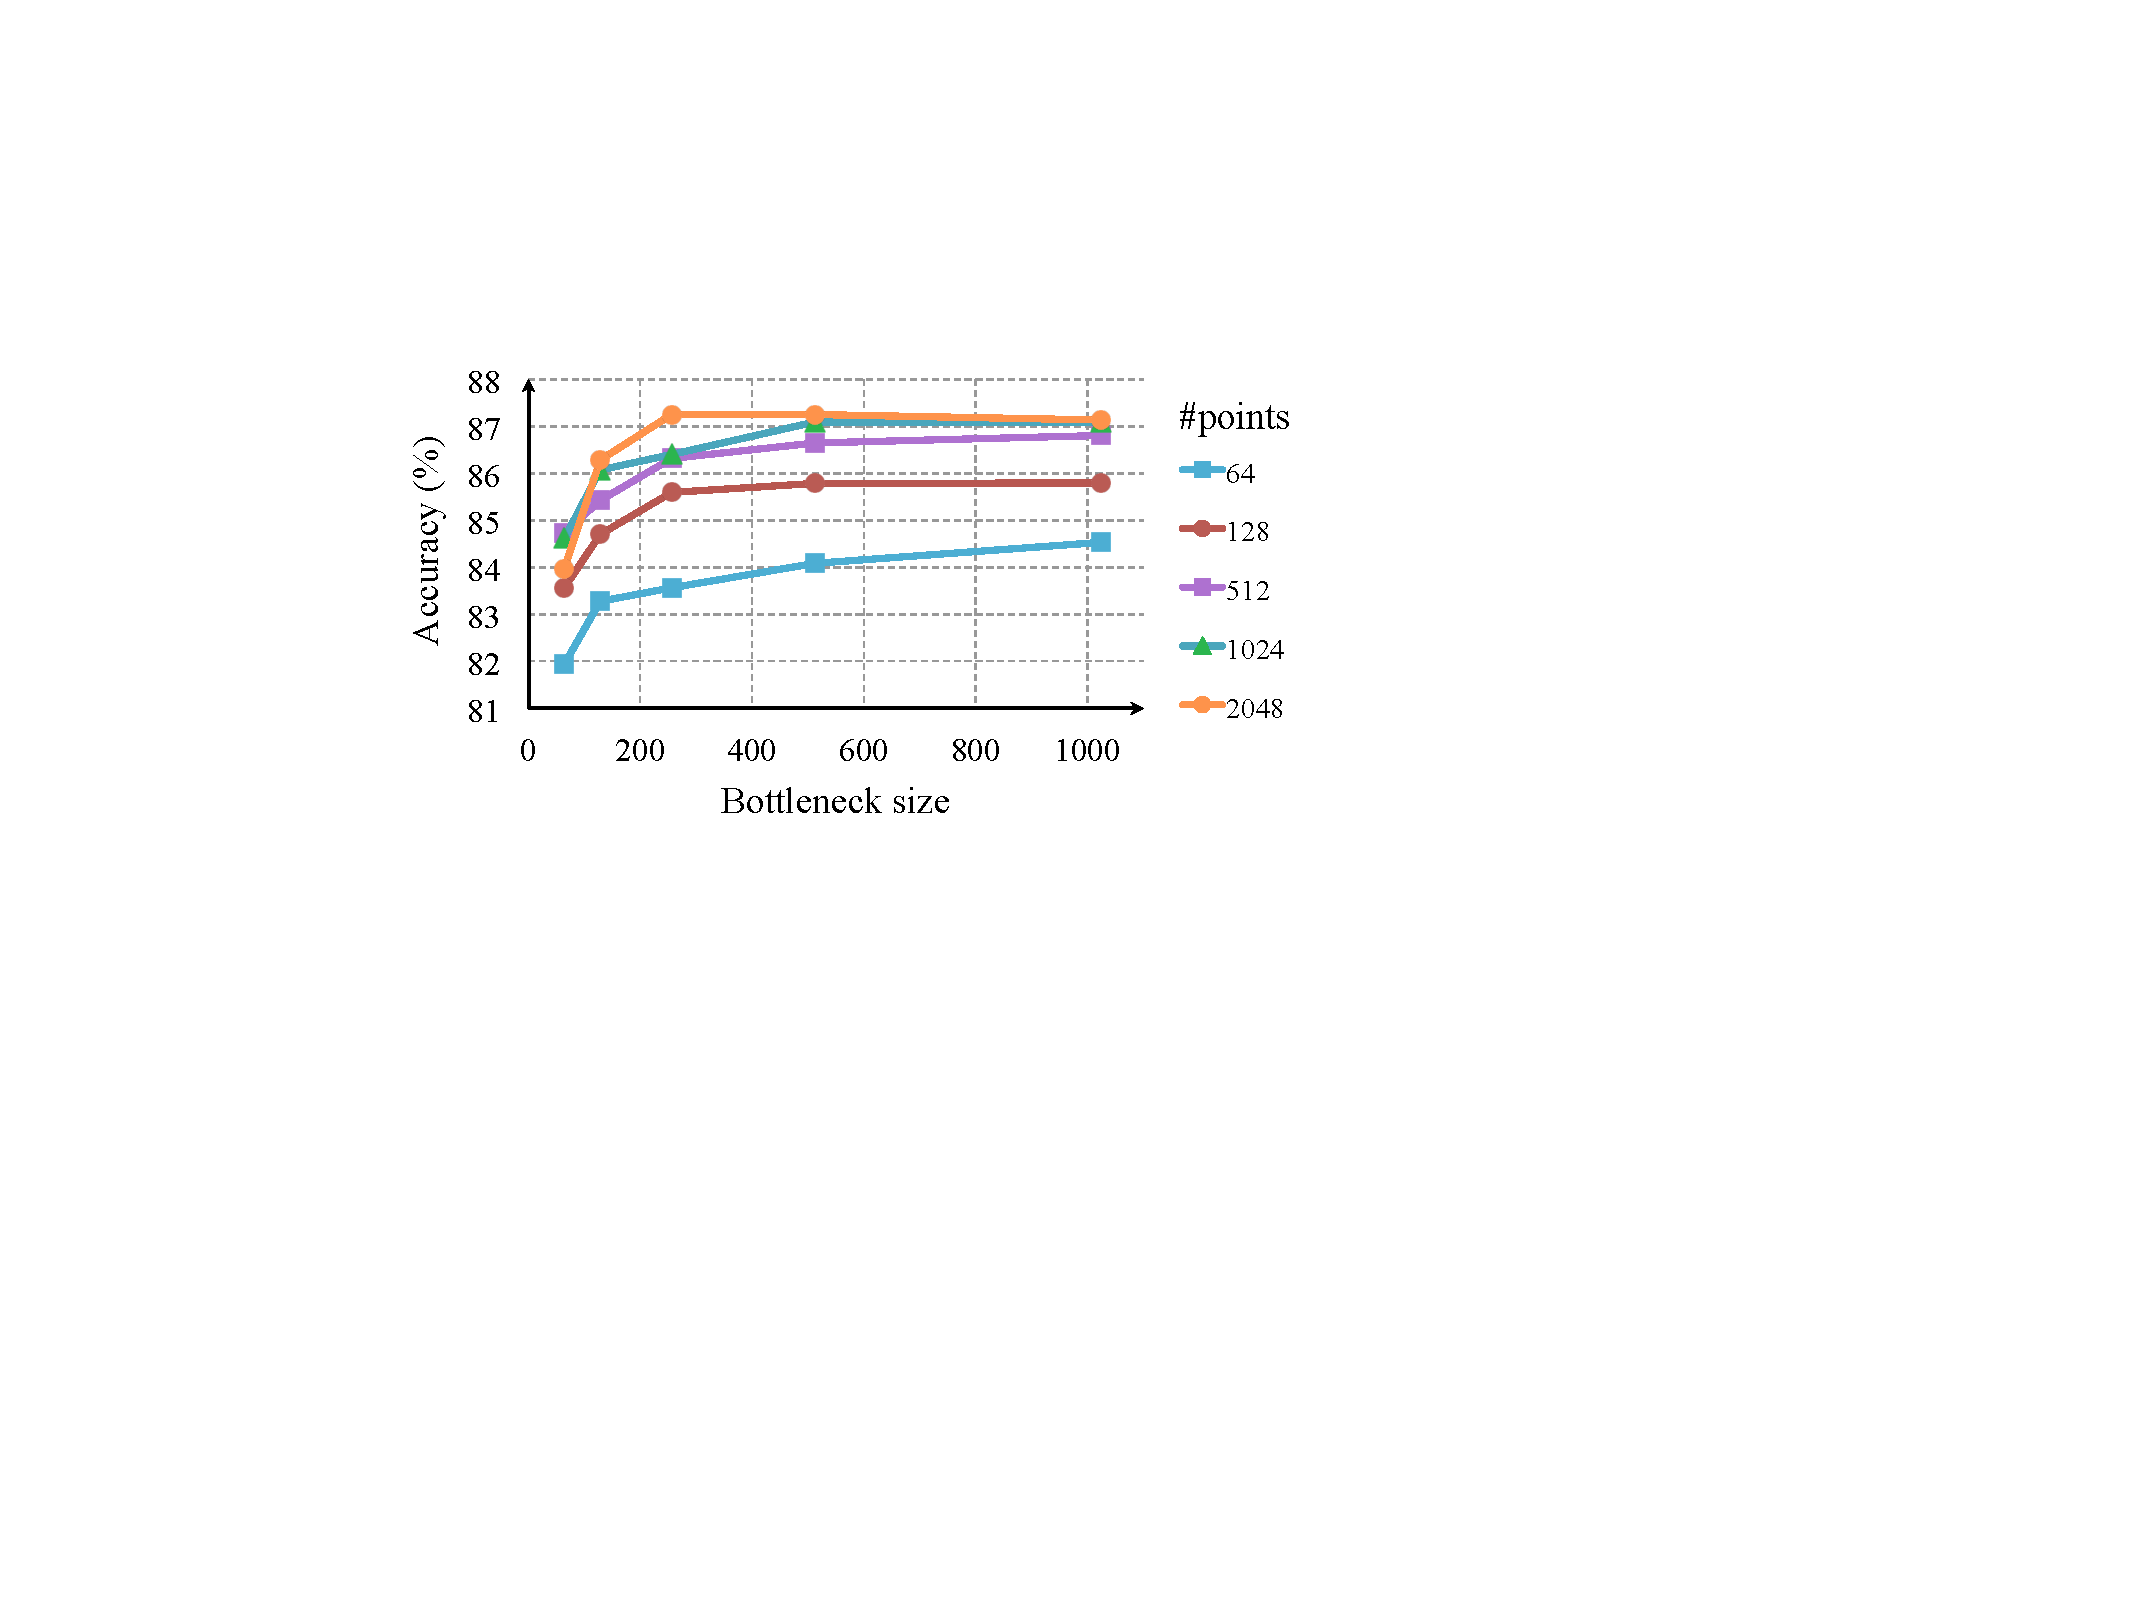
\includegraphics[width=0.8\linewidth]{fig/bottleneck.pdf}
    \caption{\textbf{瓶颈尺寸和输入点数量的效果} 该指标为 ModelNet40 上的总体的分类准确度。}
    \label{fig:net_param}
\end{figure}

\paragraph{MNIST 数字分类} 在我们关注 3D 点云的学习的同时,我们在用我们的网络在 2D 点云上做了实验,即像素集。

% \paragraph{MNIST Digit Classification}
% While we focus on 3D point cloud learning, a sanity check experiment is to apply our network on a 2D point clouds - pixel sets.

为了将一个 MNIST 图像转换成一个 2D 点云,我们设置了阈值像素值,将所有值大于 128 的像素(用图像中的 $(x,y)$ 坐标表示)加入到集合中。我们使用了一个大小为 256 的集合大小。如果集合中有多于 256 个像素,我们就从中随机地抽样;如果集合中的元素少于 256 个,我们便用集合中存在的点来做填充(由于我们的最大化操作,使用哪一个点来填充并不会影响结果)。

% To convert an MNIST image into a 2D point set we threshold pixel values and add the pixel (represented as a point with $(x,y)$ coordinate in the image) with values larger than 128 to the set. We use a set size of 256. If there are more than 256 pixels int he set, we randomly sub-sample it; if there are less, we pad the set with the one of the pixels in the set (due to our max operation, which point to use for the padding will not affect outcome).

如表 ~\ref{tab:mnist} 所示,我们将其和若干个基准线进行比较(包括将输入图像作为有序向量的多层感知机、将输入图像作为一个从 (0,0) 像素到 (27,27) 像素的循环神经网络、以及一个简易的卷积神经网络)。虽然其中表现最好的模型仍然是一个仔细调试过的卷积神经网络(达到了低于 $0.3\%$ 的错误率),但 PointNet 的表现在二维点集上的表现已经符合预期。

% As seen in Table~\ref{tab:mnist}, we compare with a few baselines including multi-layer perceptron that considers input image as an ordered vector, a RNN that consider input as sequence from pixel (0,0) to pixel (27,27), and a vanilla version CNN. While the best performing model on MNIST is still well engineered CNNs (achieving less than $0.3\%$ error rate), it's interesting to see that our PointNet model can achieve reasonable performance by considering image as a 2D point set.

% vanila CNN: https://www.microsoft.com/en-us/research/publication/best-practices-for-convolutional-neural-networks-applied-to-visual-document-analysis/

\begin{table}[h!]
    \centering
    \begin{tabular}[width=\linewidth]{l|c|c}
    \hline
    ~                      & 输入 & 错误率 (\%) \\ \hline
    多层感知机~\cite{simard2003best} & vector & 1.60  \\
    LeNet5~\cite{lecun1998gradient}                 & image & 0.80 \\ \hline
    我们的 PointNet          & point set & 0.78 \\ \hline
    \end{tabular}
    \caption{\textbf{MNIST 分类结果} 我们将我们的模型和其他简单的深度学习结构进行比对,从而说明我们的模型在二维点云上的表现仍然符合预期。
    % We compare with vanilla versions of other deep architectures to show that our network based on point sets input is achieving reasonable performance on this traditional task.
    }
    \label{tab:mnist}
\end{table}


\paragraph{法线预测}
在分割版本的 PointNet 中,为了为局部的点提供上下文信息,局部的点特征与全局的点特征被拼接在了一起。但这种拼接方式不能保证模型学习到上下文。在该实验中,我们通过展示我们的分割网络具备预测点法线(一个由某个点的邻居所决定的局部几何特征)的能力,来验证我们的设计。

% \paragraph{Normal Estimation}
% In segmentation version of PointNet, local point features and global feature are concatenated in order to provide context to local points. However, it's unclear whether the context is learnt through this concatenation. In this experiment, we validate our design by showing that our segmentation network can be trained to predict point normals, a local geometric property that is determined by a point's neighborhood.

%Our proposed PointNet learns 1024 per-point functions and uses a max-pooling operation to aggregate the per-point features into the global shape feature. Then for classification task, we push this learnt global shape signature to the subsequent classifier. The jump for per-point feature (extremely local) to the shape feature (extremely global) seems fine. However, for segmentation task, one may wonder if the local context entails crucial information to determine the local fine-grained segmentation details. Even though in our segmentation version PointNet we concatenate the learn global shape signature and the per-point local features together to do the label predictions, it is still unclear if such combination can capture the necessary local information around each point. 

我们用一种监督学习的方式修改并训练了我们的分割 PointNet 来回归到真正的点法线。我们仅仅改变了分割 PointNet 的最后一层,使其为每一个点预测法向量。对于损失函数,我们使用了余弦距离的绝对值。

% We train a modified version of our segmentation PointNet in a supervised manner to regress to the ground-truth point normals. We just change the last layer of our segmentation PointNet to predict normal vector for each point. We use absolute value of cosine distance as loss.

图 ~\ref{fig:normal_recon} 对比了我们的 PointNet 法线预测结果(左)和从网格中计算出来的真正的法线(右)。从图中可以看到,我们得到了一个合理的法线重建结果。在一些区域,我们的预测结果甚至比真正的法线(通常包括一些翻转了的法线方向)更加平滑和连续。

% Fig.~\ref{fig:normal_recon} compares our PointNet normal prediction results (the left columns) to the ground-truth normals computed from the mesh (the right columns). We observe a reasonable normal reconstruction. Our predictions are more smooth and continuous than the ground-truth which includes flipped normal directions in some region.
%Having the ability to correctly predict the point normal, one of the local geometric features that require the combination of the information of a point and its neighbors, shows our PointNet has the potential to capture the local information via simply combining the per-point feature and the aggregated global feature.

\begin{figure}[t!]
\centering
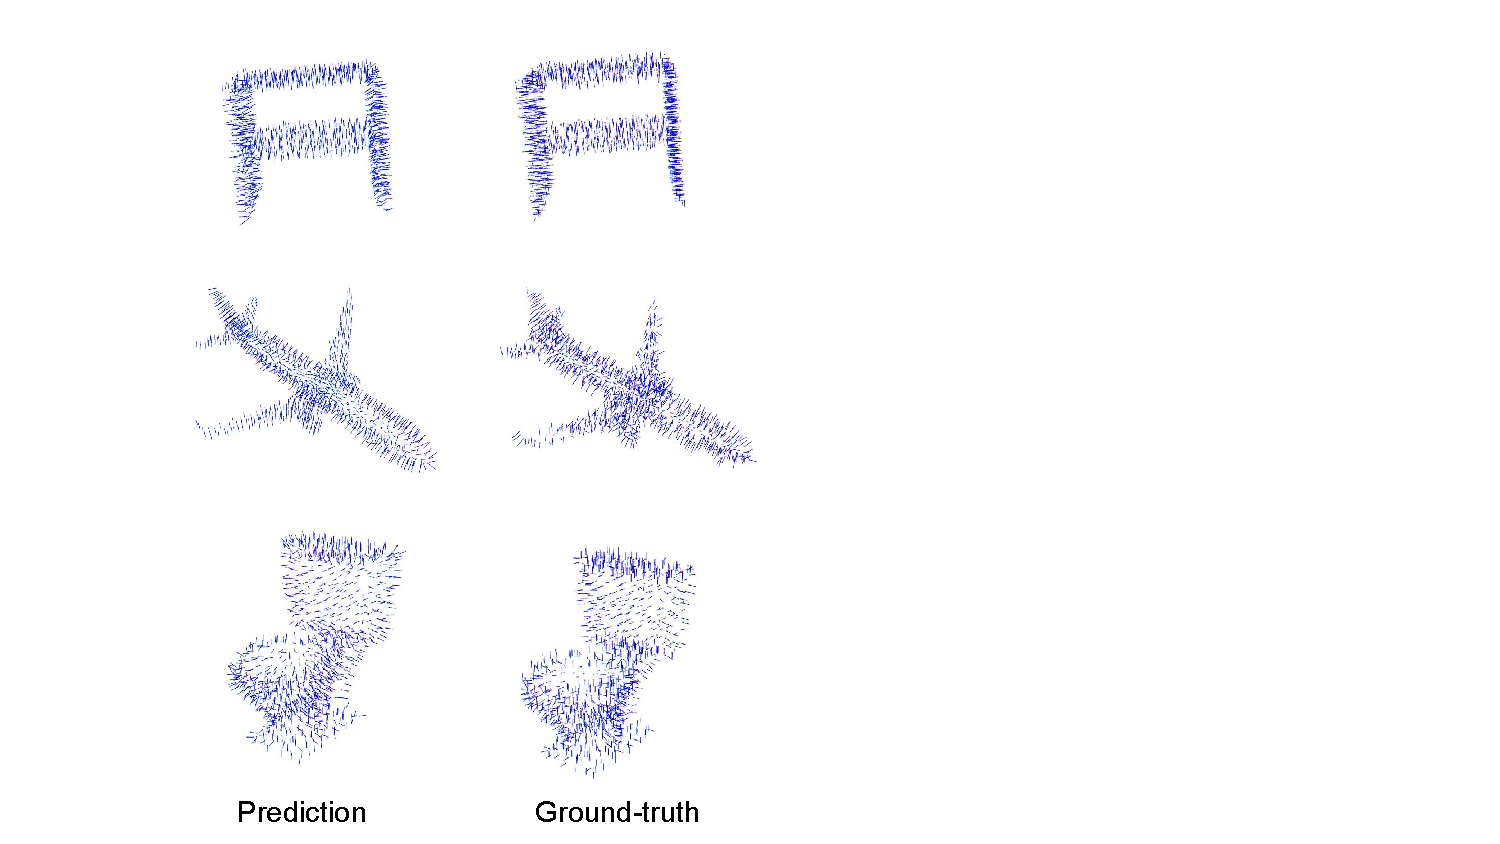
\includegraphics[width=0.9\linewidth]{fig/normal_recon2.pdf}
\caption{\textbf{PointNet 法线重建结果。} 改图展示了在一个示例点云中所有点的法线重建结果与从网格中计算出来的真正的法线结果。}
\label{fig:normal_recon}
\end{figure}


\paragraph{分割健壮性} 如 5.2 和 ~\ref{sec:cla_robust} 讨论,由于全局的形状特征是从一些 \textit{关键点} 中提取出来的,我们的点云对于数据干扰和点的缺失并不敏感。在这一部分中,我们展示了我们的模型在面对分割任务时,仍然保持着健壮性。每一个点的标签是根据两部分来预测的:各个点的特征的结合,与模型学习到的全局形状特征。在图 ~\ref{fig:seg_robust} 中,我们展示了给定输入点云 $S$ (左)的分割结果、\textit{关键点集} $\mathcal{C}_S$ (中)和 \textit{上界形状} $\mathcal{N}_S$。

% \paragraph{Segmentation Robustness} As discussed in Sec 5.2 and Sec~\ref{sec:cla_robust}, our PointNet is less sensitive to data corruption and missing points for classification tasks since the global shape feature is extracted from a collection of \textit{critical points} from the given input point cloud. In this section, we show that the robustness holds for segmentation tasks too. The per-point part labels are predicted based on the combination of per-point features and the learnt global shape feature. In Fig~\ref{fig:seg_robust}, we illustrate the segmentation results for the given input point clouds $S$ (the left-most column), the \textit{critical point sets} $\mathcal{C}_S$ (the middle column) and the \textit{upper-bound shapes} $\mathcal{N}_S$.

%One may observe that the segmentation results for the entire shape family containing all the shapes transiting between $\mathcal{C}_S$ and $\mathcal{N}_S$ are consistent, meaning that \textbf{losing some points that are not \textit{critical} does not affect the segmentation result}.

\begin{figure}[t!]
\centering
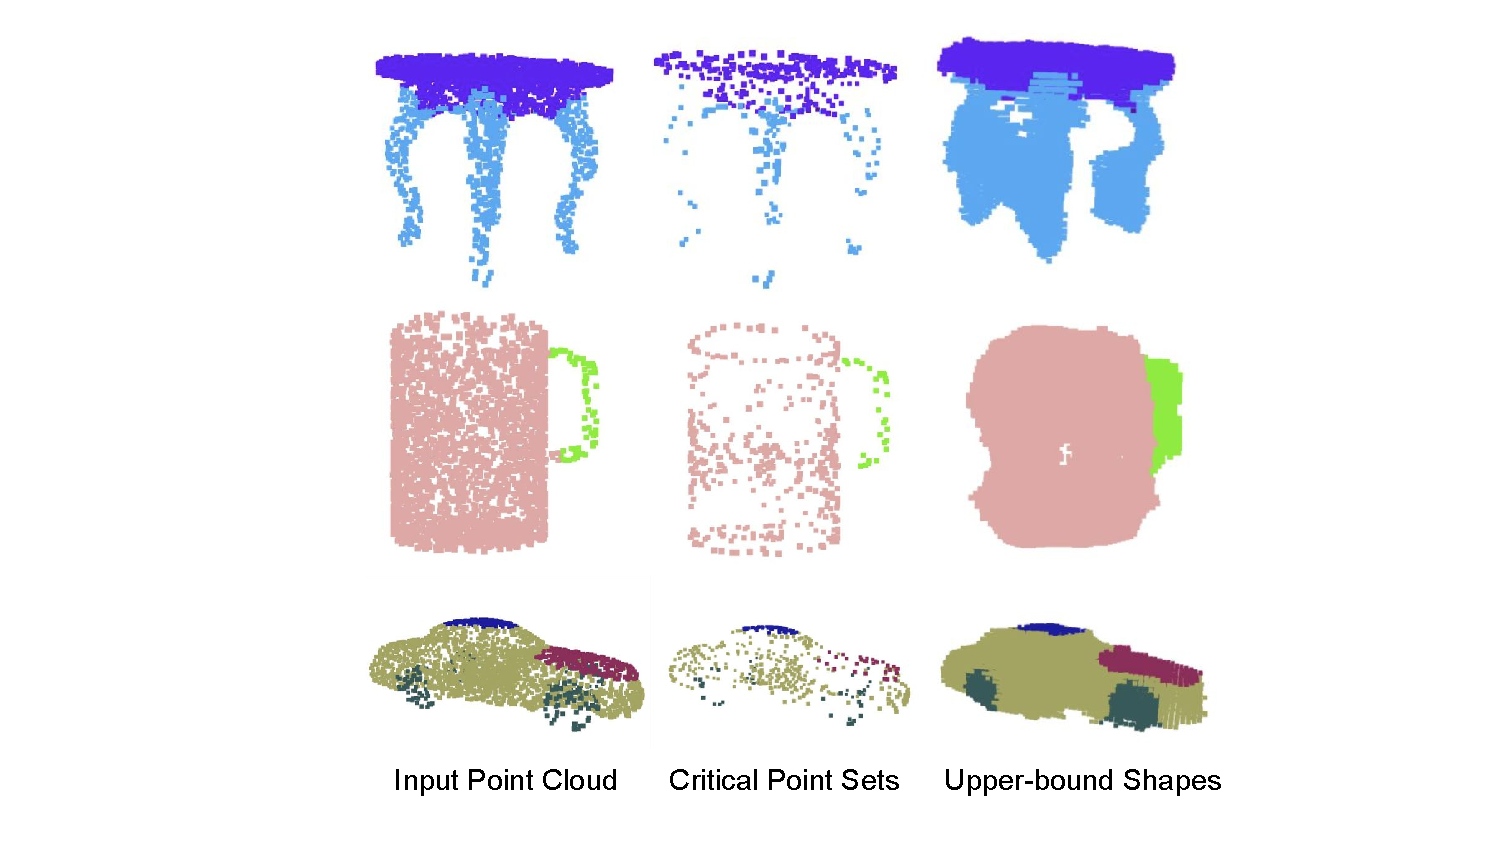
\includegraphics[width=0.9\linewidth]{fig/seg_robust.pdf}
\caption{\textbf{分割结果的一致性} 我们用图例说明一些样例物体点云的\textit{关键点集} $\mathcal{C}_S$和\textit{上界形状} $\mathcal{N}_S$ 的分割结果。 可以得出从$\mathcal{C}_S$ 到 $\mathcal{N}_S$ 的形状簇拥有共同的分割结果。}
\label{fig:seg_robust}
\end{figure}

% \begin{comment}

在 5.2 \textit{三维物体零件分割}中,我们将我们提出的 PointNet 模型应用在了 CAD 模型的语义零件分割上。我们的分割 PointNet(如图 2 \textit{分割网络})在完整的 ShapeNet 网络上达到了最优的效果。意料之中的,我们的模型在局部数据(如:模拟的 Kinect 扫描结果)中也表现的很好。由于真实世界中的扫描通常因为遮挡问题而变得十分不完整,模型在面对局部输入时的健壮性非常重要,是评估其实际应用价值的关键。表 ~\ref{tab:segmentation_partial} 概括了在面对完整的和局部的数据时,我们的 PointNet 与作为基准线的三维卷积神经网络方法得出的效果。

% In Sec 5.2 \textit{3D Object Part Segmentation}, we apply our proposed PointNet on segmenting the CAD models into semantic parts. While our segmentation PointNet (illustrated in Fig. 2, \textit{Segmentation Network}) achieves the state-of-the-art result on complete ShapeNet shapes, it performs reasonably well on partial data (e.g. simulated Kinect scans) as well. Since most real world scans are very partial due to occlusions, a model's robustness to partial input is key to evaluate its value in practice. Table~\ref{tab:segmentation_partial} summarizes the performance of our PointNet and the proposed baseline 3D CNN method when being applied to complete and partial data.


\begin{table}[h!]
    \small
    \centering
    \begin{tabular}[width=\linewidth]{l|cccc}
    \hline
    ~ & 完整输入 & 局部输入 \\ \hline
    3D CNN & 75.3 & 69.7 \\ \hline
    Ours PointNet & \textbf{80.6} & \textbf{75.3}  \\ \hline
    \end{tabular}
    \caption{\textbf{局部扫描的分割结果} 衡量指标为所有形状的 mIoU。在完整数据上训练我们的点网络时,我们进行了旋转增强,以便与从多个角度生成的模拟Kinect扫描进行公平的比较。两个网络分别在完整数据和部分数据上进行训练,然后在不同的子测试集上进行了测试。}
    \label{tab:segmentation_partial}
\end{table}

% \begin{table}[h!]
%     \small
%     \centering
%     \begin{tabular}[width=\linewidth]{l|cccc}
%     \hline
%     ~ & 完整输入 & 局部输入 \\ \hline
%     3D CNN & 75.3 & 69.7 \\ \hline
%     Ours PointNet & \textbf{80.6} & \textbf{75.3}  \\ \hline
%     \end{tabular}
%     \caption{\textbf{Segmentation results on partial scans.} Metric is mean IoU across all shapes. We perform rotation augmentation when training our PointNet on complete data to fairly compare with the simulated Kinect scans, that are generated from multiple perspective. Both networks are trained respectively on the complete data and the partial data and then tested on the testing splits.}
%     \label{tab:segmentation_partial}
% \end{table}

% \end{comment}

\paragraph{网络面对未知形状分类的通用性}
在图 \ref{fig:unseen} 中,我们可视化了 \textit{关键点集} 和 \textit{上界形状} 在面对来自从未出现在 ModelNet 或 ShapeNet 中的未知分类(脸部、马、兔子、茶壶)的新性状。结果表明,我们的模型学习到的各个点的函数是具备通用性的。然而,由于我们主要使用具备大量平面结构的人造物品来训练模型,重建出来上界形状同样也包含了更多的平面表面。

% In Fig~\ref{fig:unseen}, we visualize the \textit{critical point sets} and the \textit{upper-bound shapes} for new shapes from unseen categories (face, house, rabbit, teapot) that are not present in ModelNet or ShapeNet. It shows that the learnt per-point functions are generalizable. However, since we train mostly on man-made objects with lots of planar structures, the reconstructed upper-bound shape in novel categories also contain more planar surfaces. 
 


% \paragraph{Network Generalizability to Unseen Shape Categories}
% %As discussed in the previous sections, our proposed PointNet learns several useful per-point functions and computes the global shape signature by max pooling all the point features.
% %In Sec 5.3, we visualize the learnt per-point functions and observe that they work in the way to detect if some points intersect with some specific regions. And, by aggregating the learnt per-point features, PointNet selects some \textit{critical points} and produces the global shape feature by summarizing the activation values of them.
% In Fig~\ref{fig:unseen}, we visualize the \textit{critical point sets} and the \textit{upper-bound shapes} for new shapes from unseen categories (face, house, rabbit, teapot) that are not present in ModelNet or ShapeNet. It shows that the learnt per-point functions are generalizable. However, since we train mostly on man-made objects with lots of planar structures, the reconstructed upper-bound shape in novel categories also contain more planar surfaces. 
 
\begin{figure}[t!]
\centering
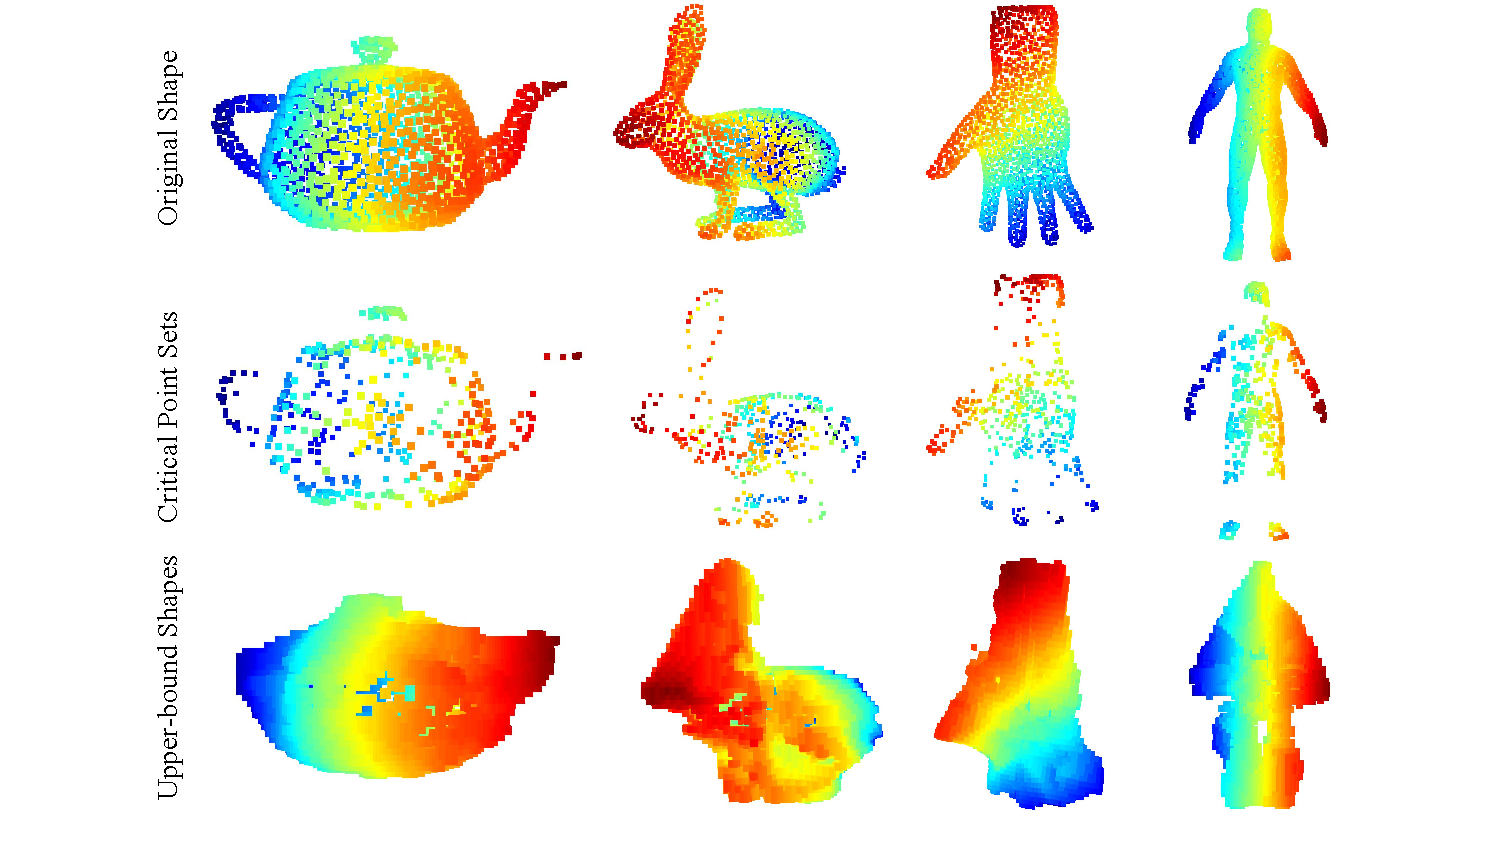
\includegraphics[width=\linewidth]{fig/unseen.pdf}
\caption{\textbf{未知物体的关键点集和上界形状} 我们可视化了茶壶,兔子,手,人体的 \textit{关键点集} 和 \textit{上界形状}。 通过这些不在ModelNet和ShapeNet数据集的物体来测试PointNet学习到的点函数的通用性。图中用颜色编码反应深度信息。}
\label{fig:unseen}
\end{figure}

\section{定理证明 (Sec 4.3)}
\label{sec:proof}
令 $\mathcal{X}=\{S: S\subseteq [0,1]\mbox{ and } |S|=n \}$. 

若以下条件满足,则$f:\mathcal{X}\rightarrow \mathbb{R}$ 是一个$\mathcal{X}$上关于赫斯多夫距离$d_H(\cdot, \cdot)$的连续函数

$\forall \epsilon > 0, \exists \delta >0$, 对于任意一个 $S, S'\in\mathcal{X}$, if $d_H(S, S') < \delta$, then $|f(S)-f(S')|< \epsilon$.

我们证明了 $f$ 可以被对称函数和连续函数的复合函数任意逼近

% \begin{theorem}
\begin{customthm}{1}
假设 $f:\mathcal{X}\rightarrow \mathbb{R}$ 是一个关于赫斯多夫距离$d_H(\cdot, \cdot)$的连续集函数。 $\forall \epsilon > 0$, $\exists$ 一个连续函数 $h$ 和一个对称函数 $g(x_1, \dots, x_n)=\gamma \circ \mbox{MAX}$, 其中 $\gamma$ 一个连续函数, $\mbox{MAX}$是一个取 $n$ 个向量最为输入,然后返回一个元素层面上的最大值的最大化向量运算符, 对于任意一个 $S\in\mathcal{X}$,
% Formally, $\forall \epsilon > 0$, $\exists g_{\epsilon}:\underbrace{\R^{K_\epsilon}\times \dots \times \R^{K_\epsilon}}_n\rightarrow \R$ which is a symmetric function and $h_{\epsilon}: \R^3 \rightarrow \R^{K_\epsilon}$ such that 
\begin{align*}
	|f(S) - \gamma(\mbox{MAX}(h(x_1), \ldots, h(x_n)))| < \epsilon
\end{align*}
其中 $x_1, \ldots, x_n$ 是按指定顺序从 $S$ 中提取的元素。
\end{customthm}
%\end{theorem}

\begin{proof}
通过 $f$ 的连续性, 引入 $\delta_{\epsilon}$ 来说明 
$|f(S)-f(S')|<\epsilon$ 对于任意一个 $S, S'\in \mathcal{X} \mbox{ if } d_H(S, S')<\delta_{\epsilon}$. 

定义 $K=\lceil 1/\delta_{\epsilon}\rceil$, 将 $[0,1]$ 均分成 $K$ 个间隔,同时定义辅助函数,将点映射到它所在间隔的左端:
$$\sigma(x)=\frac{\lfloor K x \rfloor}{K}$$
令 $\tilde{S}=\{\sigma(x):x\in S\}$
$$|f(S)-f(\tilde{S})|< \epsilon$$
因为 $d_H(S, \tilde{S})<1/K\le \delta_{\epsilon}$.

令 $h_k(x)=e^{-d(x, [\frac{k-1}{K}, \frac{k}{K}])}$ 为一个轻指示函数,其中 $d(x, I)$ 是点的间隔距离。 令 $\myvec h(x)=[h_1(x); \ldots; h_K(x)]$,  $\myvec h:\mathbb{R}\rightarrow \mathbb{R}^K$. 

令 $v_j(x_1, \ldots, x_n)=\max\{\tilde{h}_j(x_1),\ldots,\tilde{h}_j(x_n)\}$ 代表第$j$-th区间中$S$中点的占比。 令 $\myvec v=[v_1;\ldots; v_K]$, $\myvec v:\underbrace{\mathbb{R}\times \ldots\times \mathbb{R}}_{n}\rightarrow \{0, 1\}^K$ 是一个对称函数, 代表每个区间中$S$中点的占比。

定义 $\tau:\{0, 1\}^K\rightarrow \mathcal{X}$ 为 $\tau(v)=\{\frac{k-1}{K}: v_k\ge 1\}$, 代表占用向量到表示每个占用区间左端集合的映射。 易得:
\begin{align*}
\tau(\myvec v(x_1, \ldots, x_n))\equiv \tilde{S} 
\end{align*}
其中 $x_1, \ldots, x_n$ 是按指定顺序从 $S$ 中提取的元素。

令 $\gamma:\mathbb{R}^K\rightarrow \mathbb{R}$ 为一个连续函数,对于 $v\in\{0, 1\}^K$ 有 $\gamma(\myvec v)=f(\tau(\myvec v))$ 对于 $v\in\{0, 1\}^K$. 则
\begin{align*}
&|\gamma(\myvec v(x_1, \ldots, x_n))-f(S)|\\
=&|f(\tau(\myvec v(x_1, \ldots, x_n)))-f(S)|<\epsilon
\end{align*}

注意 $\gamma(\myvec v(x_1, \ldots, x_n))$ 可以被写成以下形式:
\begin{align*}
\gamma(\myvec v(x_1, \ldots, x_n))=&\gamma(\mbox{MAX}(\myvec h(x_1), \ldots, \myvec h(x_n)))\\
=&(\gamma \circ \mbox{MAX}) (\myvec h(x_1),\ldots,\myvec h(x_n))
\end{align*}
显然 $\gamma \circ \mbox{MAX}$ 是一个对称函数。
% $f(\tau(\myvec v(x_1,\ldots, x_n)))$. Clearly, $\gamma$ is a piece-wise constant function. Due to the universal approximation property of neural networks, 
\end{proof}

接下来给出定理2的证明。
定义 $\myvec u=\underset{x_i\in S}{\mbox{MAX}}\{h(x_i)\}$ 为$f$的子网络,表示$[0,1]^m$上点集到$K$-维向量的映射。以下定理表明输入点集中较少点缺失或者额外微小点扰动不会改变我们网络的输出:
% \begin{theorem}
\begin{customthm}{2}
假设 $\myvec u:\mathcal{X}\rightarrow \mathbb{R}^K$ 其中 $\myvec u=\underset{x_i\in S}{\mbox{MAX}}\{h(x_i)\}$ 且 $f=\gamma \circ \myvec u$. 则, 
\begin{enumerate}[label=(\alph*)]   
    \item $\forall S, \exists~\mathcal{C}_S, \mathcal{N}_S\subseteq \mathcal{X}$,  $f(T)=f(S)$ if  $\mathcal{C}_S\subseteq T\subseteq \mathcal{N}_S$;
    %\item Define the equivalence relation $\sim$ as $S\sim S'$ if $\myvec u(S)=\myvec u(S')$, then $\mathcal{C}_S=\underset{S'\sim S}{\cap} S'$ and $\mathcal{N}_S=\underset{S'\sim S}{\cup} S'$.
    % \item Let $S\sim S'$ if $\myvec u(S)=\myvec u(S')$. $\mathcal{C}_S=\underset{S'\sim S}{\cap} S'$, $\mathcal{N}_S=\underset{S'\sim S}{\cup} S'$.
    \item $|\mathcal{C}_S| \le K$
\end{enumerate}
%\label{thm:thm2}
%     \begin{itemize}            
%     \item Critical points.
%     \\$\mathbb{C}=\{x_i: \myvec u_j(S)=h_j(x_i) \mbox{ for some } 1\le j\le K\}\cap S$
%     \item Free-space points.
%     \\$\mathbb{F}=\{x_i: \myvec u_j(S)<h_j(x_i) \mbox{ for some } 1\le j\le K\}\cap S$
%     \item Non-critical points. 
%     \\$\mathbb{N}=\{x_i: \myvec u_j(S)>h_j(x_i) \mbox{ for some } 1\le j\le K\}\cap S$
% For any $S'$ such that  $\mathbb{C} \subseteq S' \subseteq \mathbb{C}\cup\mathbb{N}$, $\myvec u(S')\equiv \myvec u(S)$; for any $S'$ such that $S'\cap \mathbb{F}\neq \emptyset$, $\myvec u(S')\neq \myvec u(S)$.
%\end{itemize}
\end{customthm}
%\end{theorem}
\begin{proof}
显然, $\forall S\in \mathcal{X}$, $f(S)$ 由$\myvec u(S)$所决定。所以我们只需要证明 
$\forall S, \exists\,\mathcal{C}_S, \mathcal{N}_S\subseteq \mathcal{X}, f(T)=f(S)\,\mbox{if}\,\mathcal{C}_S\subseteq T\subseteq \mathcal{N}_S$. 

对于输出向量$\myvec u$的第$j$维 , 存在至少一个 $x_j \in \mathcal{X}$ 使得 $h_j(x_j)=\myvec u_j$, 其中 $h_j$ 是$h$中第$j$维输出向量。 将 $\mathcal{C}_S$ 作为所有$x_j$ , $j=1,\ldots,K$ 的聚合,则 $\mathcal{C}_S$ 满足上述条件。

因此对于$f$,附加任意额外的点$x$使得$\mathcal{C}_S$的每一维满足$h(x)\le \myvec u(S)$ 而不改变$\myvec u$。从而得出,可以把所有这样点添加到$\mathcal{N}_S$来得到$\mathcal{T}_S$。




\end{proof}


\begin{figure}[h!]
    \centering
    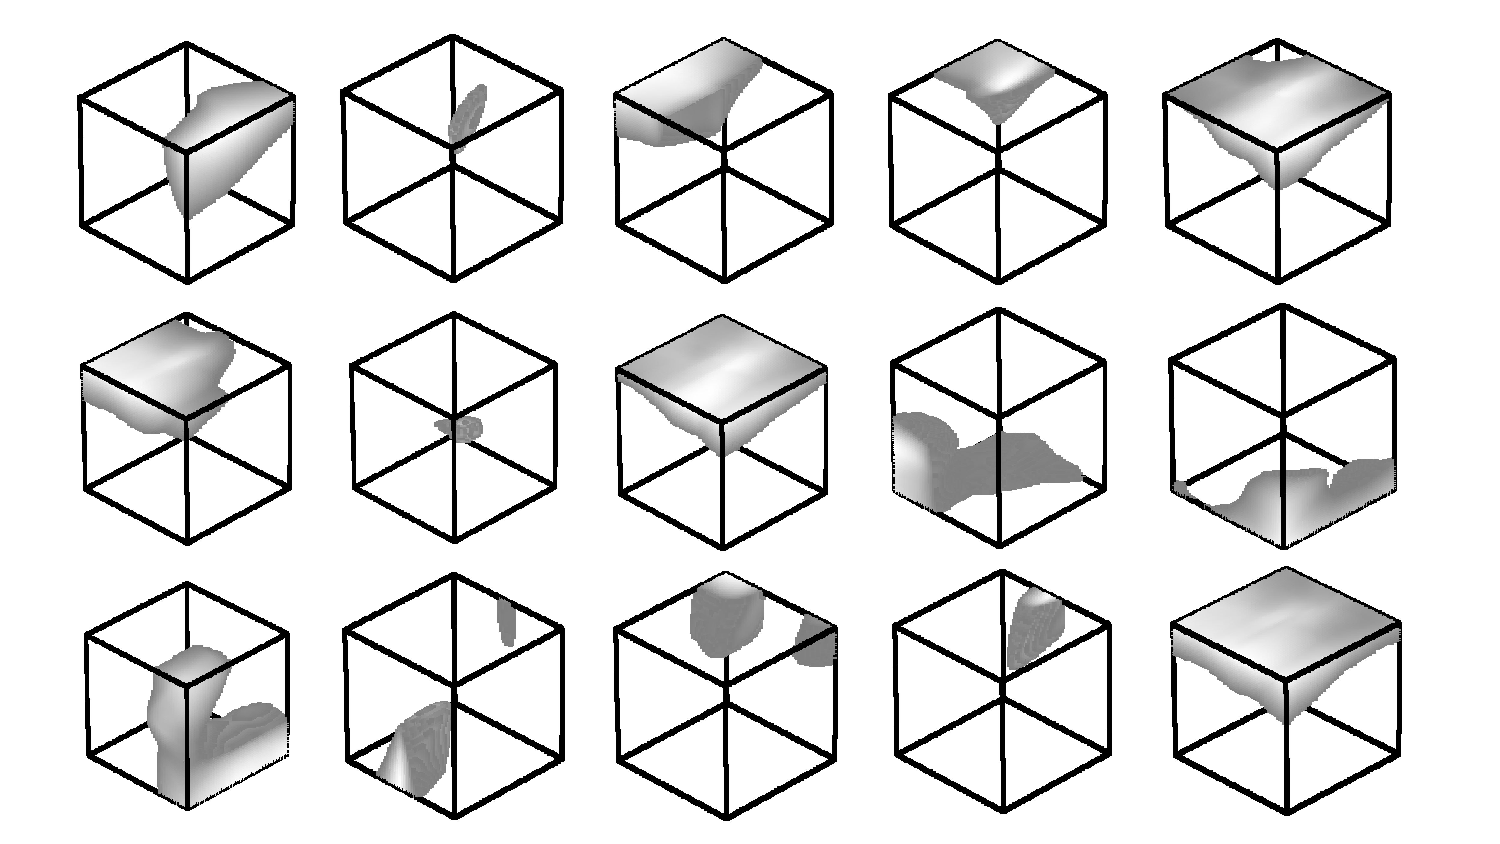
\includegraphics[width=0.7\linewidth]{fig/kernels.pdf}
    \caption{\textbf{点函数可视化} 对于每个点函数$h$,计算位于原点的边长为2的立方体中每个点$p$的$h(p)$值 , 该区域覆盖了训练PointNet时输入数据规范化的单位球区域。 在这幅图中, 我们可视化所有$h(p)>0.5$的点$p$,函数值用体素亮度表示。 我们随机选取15个点函数并可视化其活跃区域。}
    \label{fig:functions}
\end{figure}

\section{更多的可视化}
\label{sec:visu}
\paragraph{分类可视化}
%In this section, we investigate the classification version PointNet, visualize the shape global feature space via 2D embedding and provide some error analysis on the failure cases.

我们使用t-SNE\cite{maaten2008visualizing}把从我们的分类PointNet中得到的点云全局结果(1024-dim)降维嵌入到2D空间中。图~\ref{fig:tsne}显示了ModelNet40用于测试的分割形状的嵌入空间。相似的形状根据它们的语义类别分别聚集到一起。

\begin{figure*}[t!]
\centering
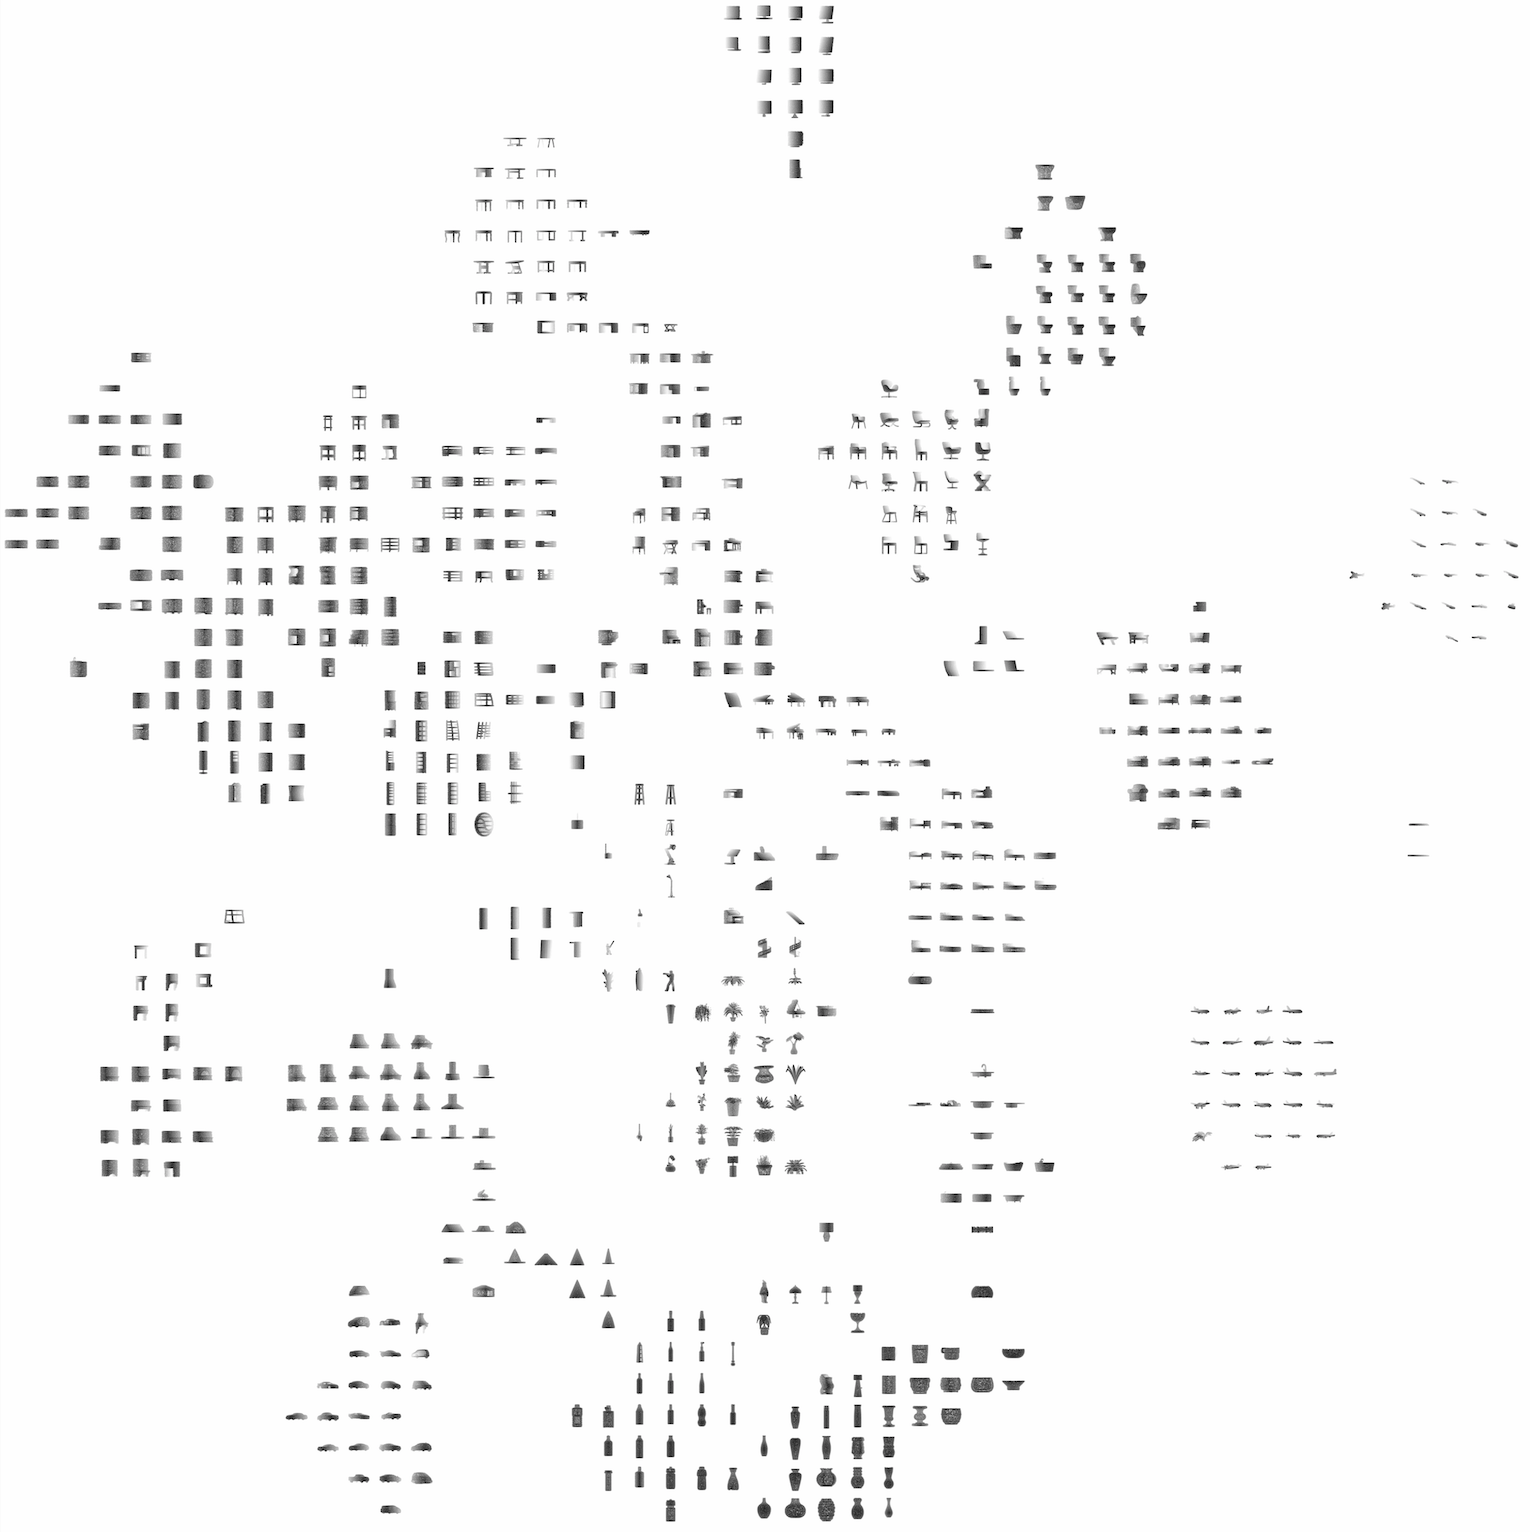
\includegraphics[width=\linewidth]{fig/tsne.png}
\caption{\textbf{所学到的形状全局特征的二维嵌入}我们使用t-SNE技术将学习到的全局形状特征可视化为ModelNet40测试时拆分的形状。}
\label{fig:tsne}
\end{figure*}


\paragraph{分割可视化} 我们在完整的CAD模型和模拟Kinect部分扫描上提供了更多的分割结果。我们还可视化了具有错误分析的失败案例。 图~\ref{fig:part_seg_complete} 和 图~\ref{fig:part_seg_partial} 显示了在完整CAD模型及其模拟Kinect扫描上生成的更多分割结果。 图~\ref{fig:part_seg_failure} 说明了一些失败案例情况。请阅读错误分析的说明。

\begin{figure*}[t!]
\centering
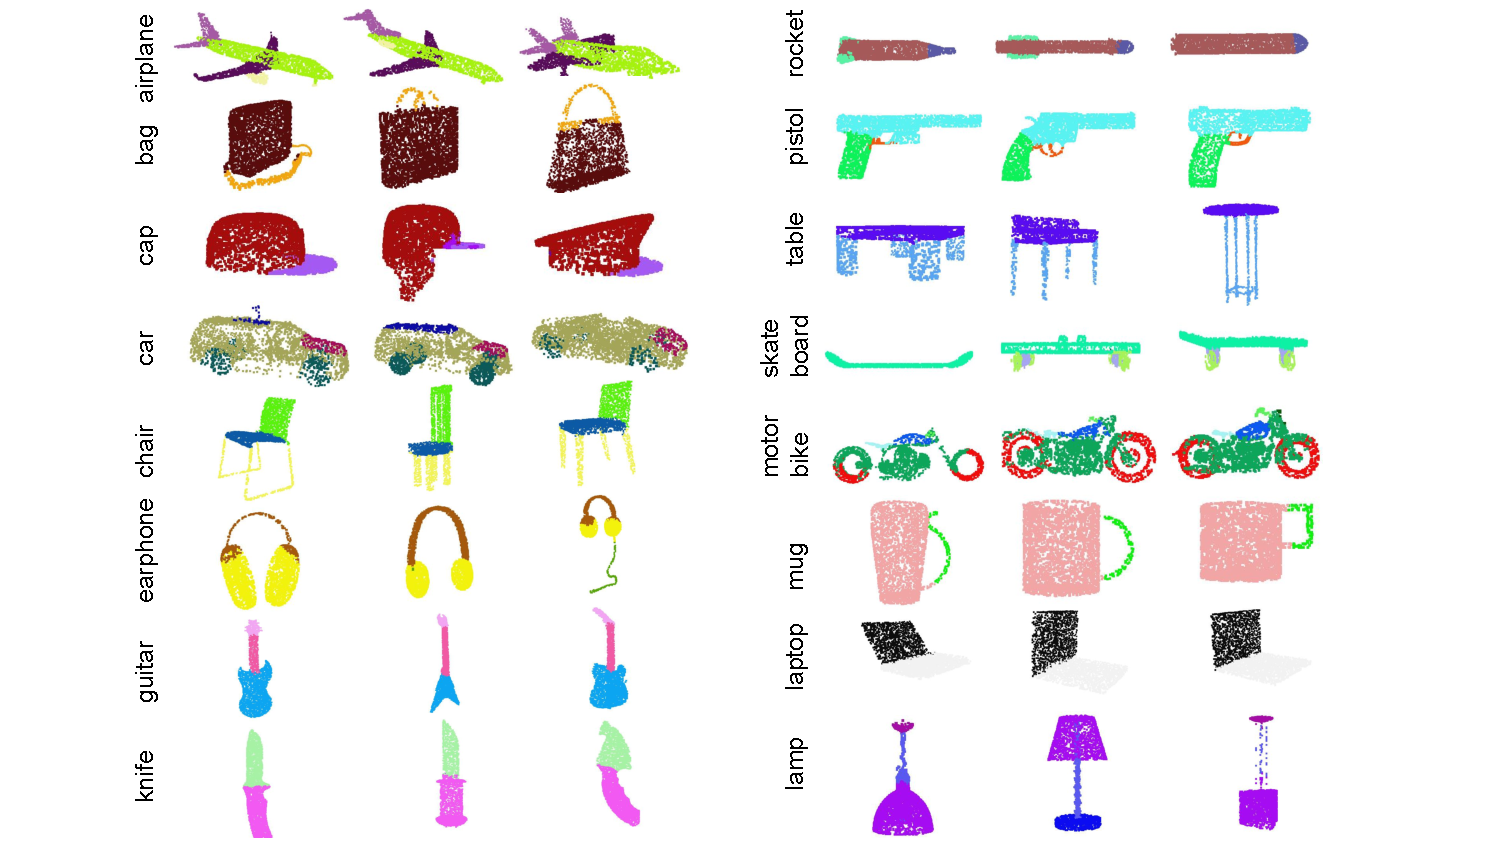
\includegraphics[width=0.82\linewidth]{fig/part_seg_complete.pdf}
\caption{\textbf{PointNet在完整的CAD模型上的分割结果} }
\label{fig:part_seg_complete}
\end{figure*}

\begin{figure*}[t!]
\centering
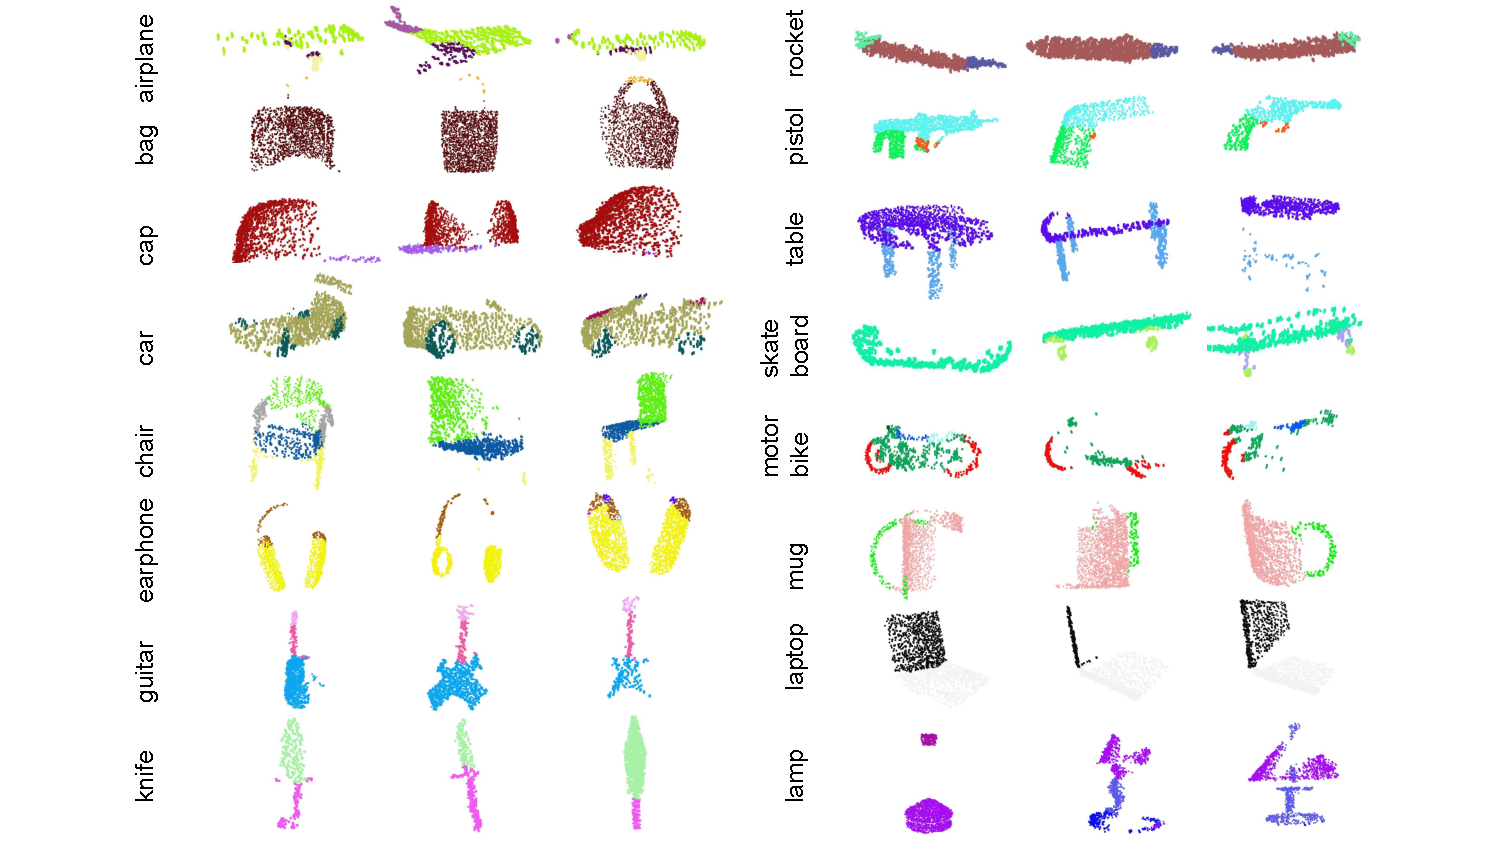
\includegraphics[width=0.82\linewidth]{fig/part_seg_partial.pdf}
\caption{\textbf{PointNet在模拟Kinect扫描上的分割结果} }
\label{fig:part_seg_partial}
\end{figure*}

\begin{figure*}[t!]
\centering
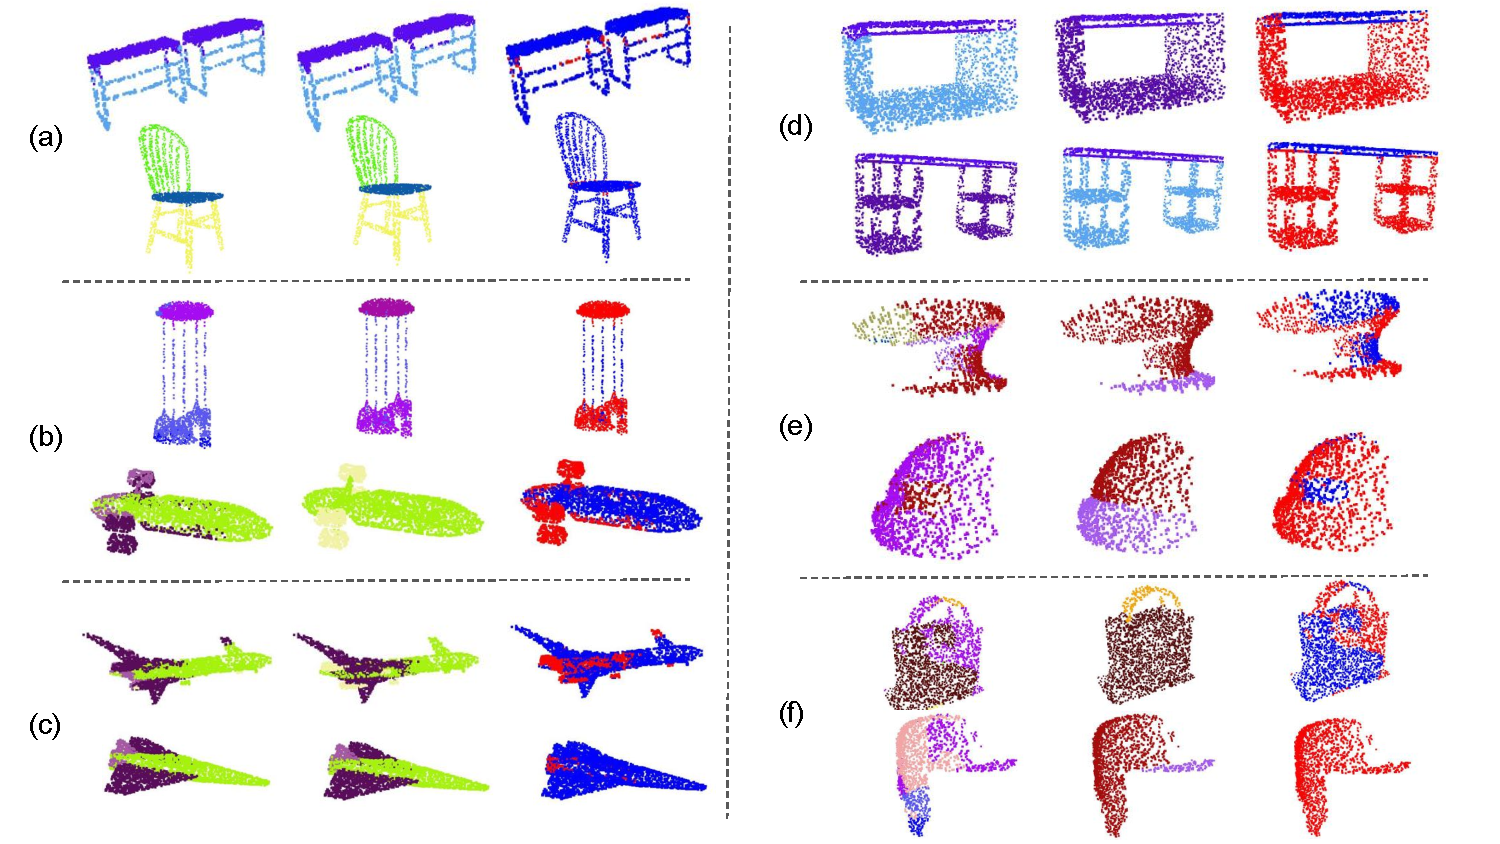
\includegraphics[width=\linewidth]{fig/part_seg_failure.pdf}
\caption{\textbf{PointNet分割失败案例} 在此图中,我们总结了分割应用程序中的六种常见错误。在第一列和第二列中分别给出了预测和真实分割结果,而差异图经计算后显示在第三列。红点对应于给定点云中标记错误的点。(a)说明了最常见的失败案例:边界上的点被错误标记。在示例中,桌椅腿和顶部之间的交叉线附近的点的标签预测不准确。然而,大多数分割算法都存在这个错误。(b)显示了奇怪形状的错误。例如,图中所示的吊灯和飞机在数据集中非常少见。(c)表明小部分可以被附近的大部分覆盖。例如,飞机的喷气发动机(图中黄色)被错误地分类为机身(绿色)或机翼(紫色)。(d)显示了由形状部分固有的模糊性引起的错误。例如,图中两张桌子的两个底部被分类为桌腿和桌脚 (\cite{Yi16}中的\textit{其他}类别),而真实分割则是相反的。(e)显示了由部分扫描的不完整性导致的错误。对于图中的两个帽子,几乎一半的点云都缺失了。(f)显示了当某些目标类别的训练数据太少而无法涵盖足够多样性时产生的失败案例。对于此处显示的两个类别,整个数据集中只有54个袋子和39个帽子。}
\label{fig:part_seg_failure}
\end{figure*}

\paragraph{场景语义解析可视化}
我们在图~\ref{fig:semantic_large} 中给出了语义解析的可视化,其中我们显示了对应两个办公室和一个会议室,用于语义分割和目标检测的输入点云、预测和真实标签。该区域和房间在训练集中是不可见的。


\begin{figure*}
    \centering
    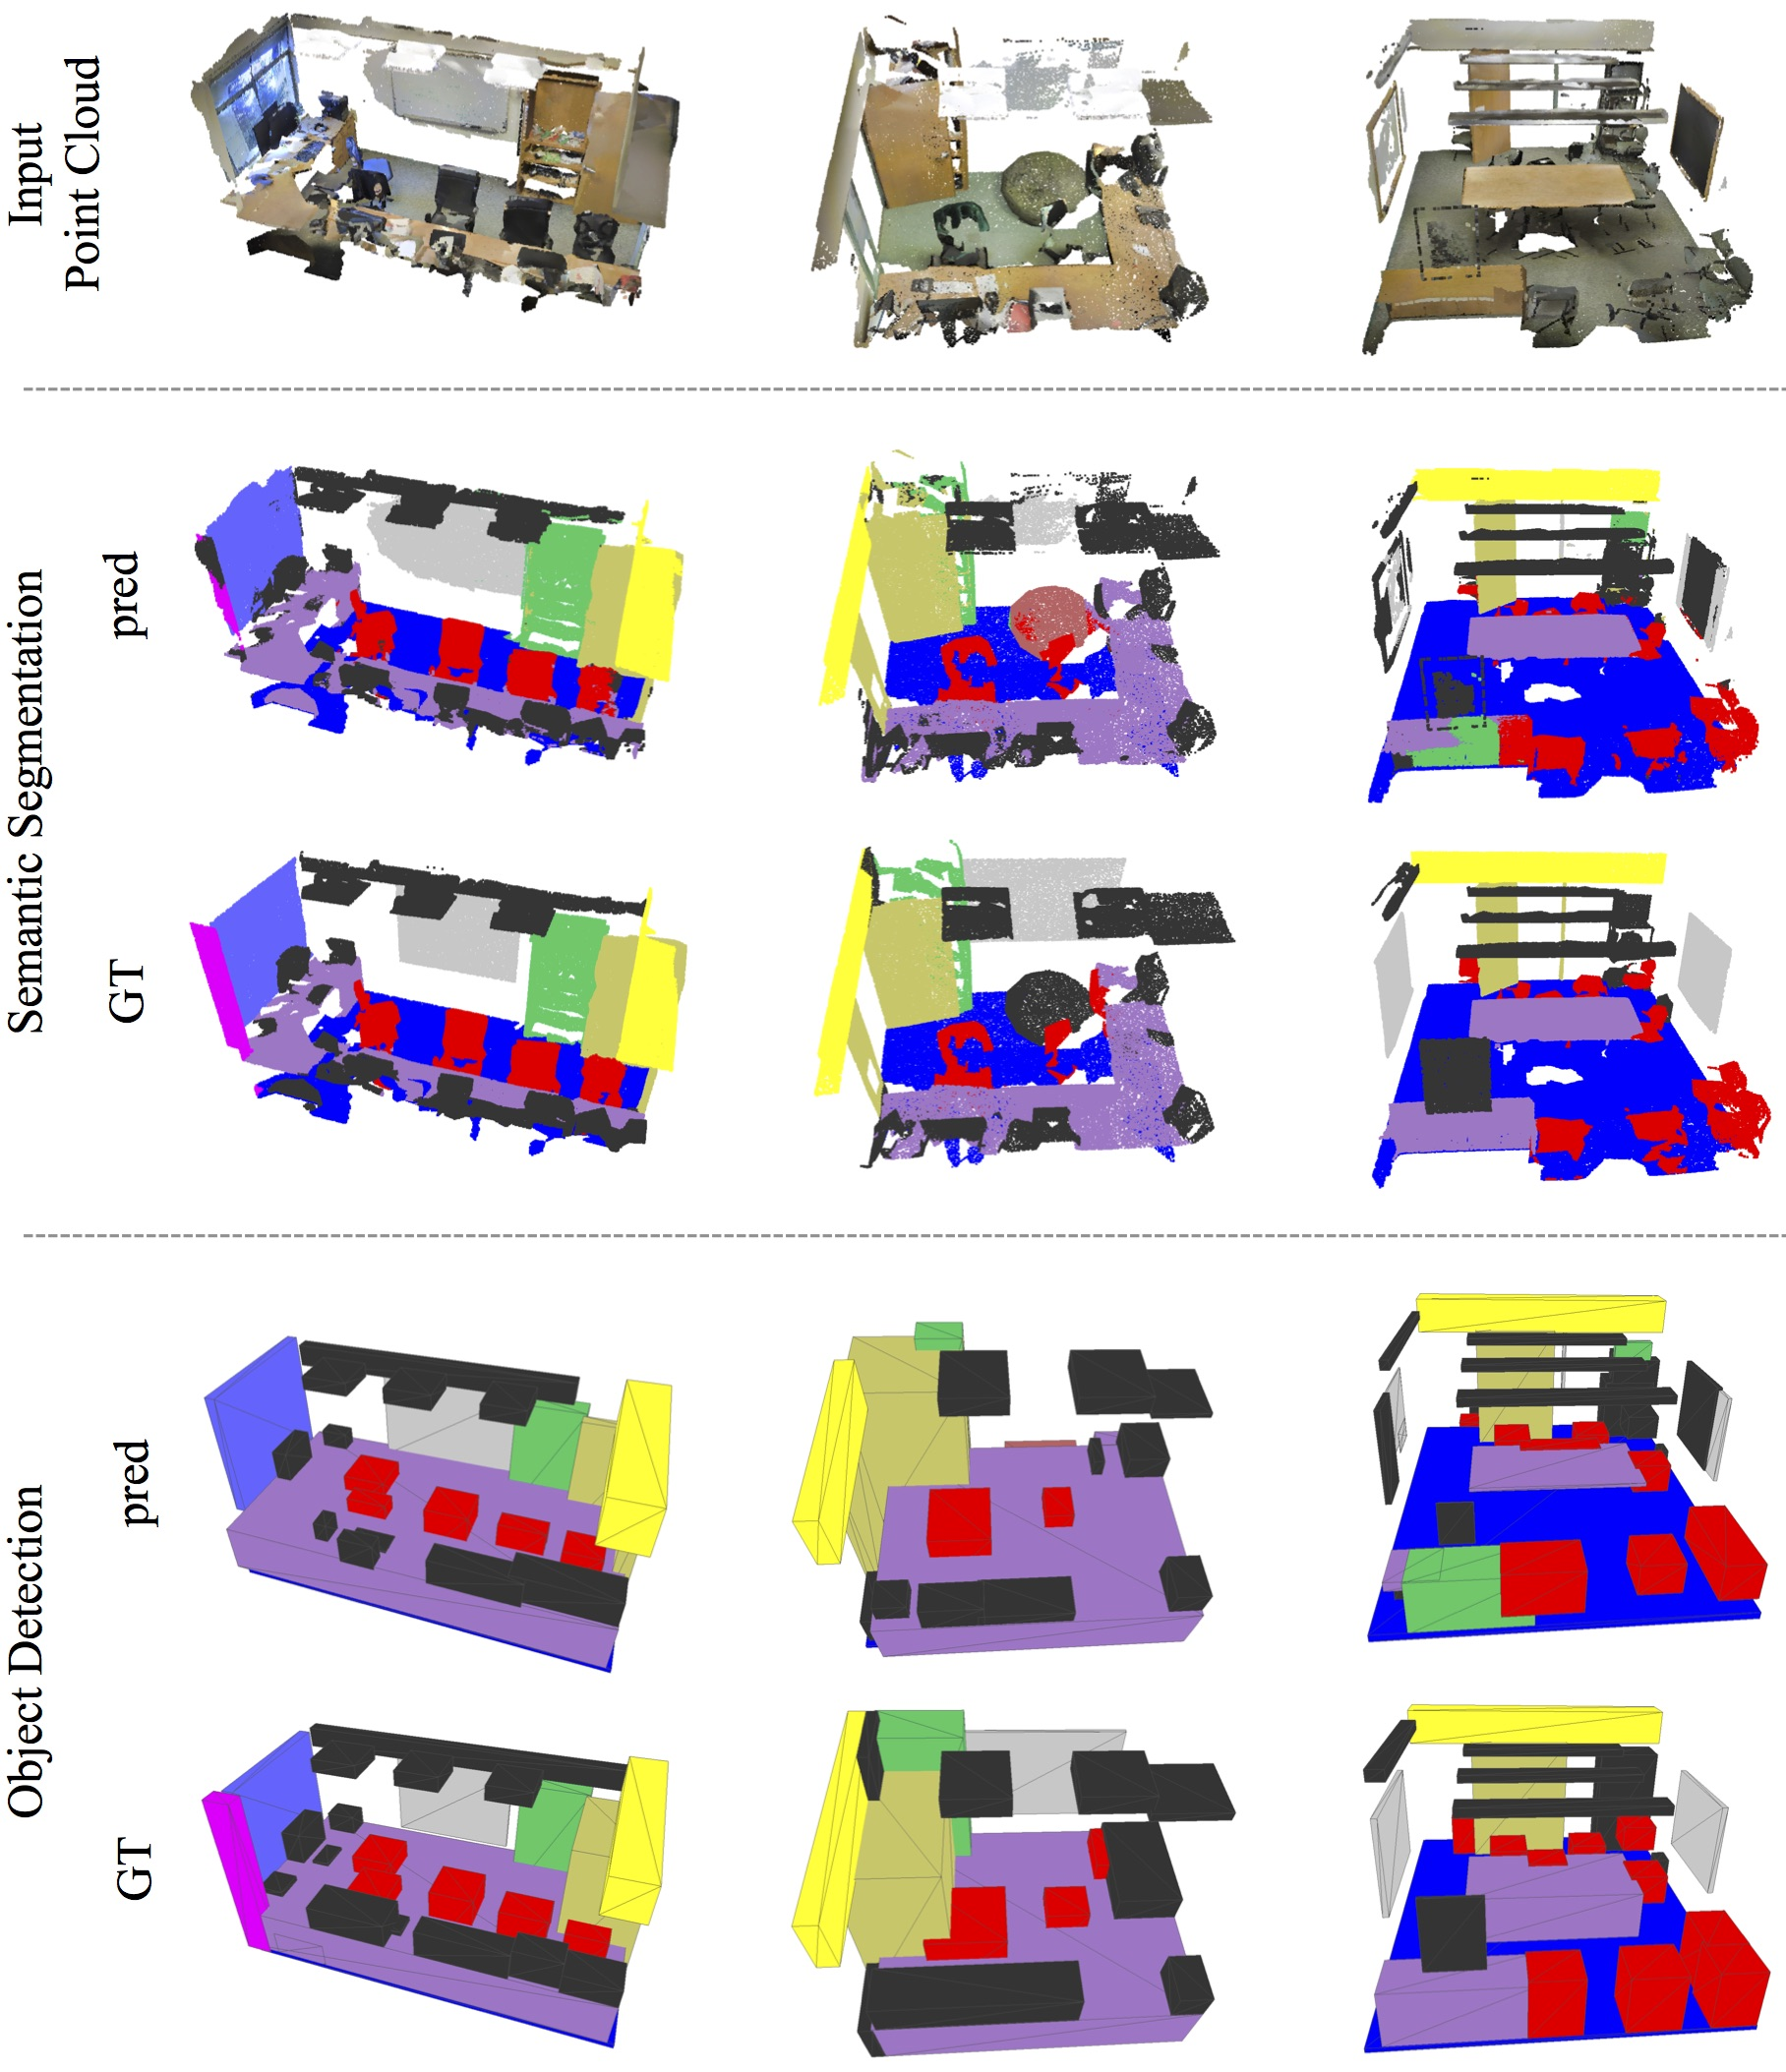
\includegraphics[width=\linewidth]{fig/semantic_large.jpg}
    \caption{\textbf{语义分割和目标检测示例}    第一行是输入点云,为了清晰度,其中墙壁和天花板被隐藏了。第二行和第三行分别是对点的语义分割的预测和真实分割,其中属于不同语义区域的点的颜色不同(椅子为红色,桌子为紫色,沙发为橙色,木板为灰色,书柜为绿色,地板为蓝色,窗户为紫色,横梁为黄色,柱子为洋红色,门为卡其色和杂物为黑色)。最后两行是带有边界框的目标检测,其中预测框来自基于语义分割预测的连接部分。}
    \label{fig:semantic_large}
\end{figure*}

\paragraph{点函数可视化} 我们的分类PointNet为每个点计算 $K$ (我们在此可视化中取 $K=1024$) 维的点特征,并通过最大池化层将所有每点局部特征聚合为单个 $K$维向量,从而形成全局形状描述符。

为了更深入地了解每个已经训练好的点函数 $h$ 所检测的内容。我们在图~\ref{fig:functions} 中可视化了具有较高的点函数值 $f(p_i)$ 的点 $p_i$。该可视化清晰地表明,不同的点函数能够会检测分散在整个空间中的不同区域中形状各异的点。


% \paragraph{Global Feature Visualization} In Fig~\ref{fig:kp_ss_visu}, we visualize more results of the \textit{critical point sets} $\mathcal{C}_S$ and the \textit{upper-bound shapes} $\mathcal{N}_S$ for some sample shapes $S$. The point sets between the two shapes will give exactly the same global shape feature $f(S)$. 

% We can see clearly from Fig~\ref{fig:kp_ss_visu} that the \textit{critical point sets} $\mathcal{C}_S$ summarizes the skeleton of the shape.
% %, or sample a sparse collection of points to describe the geometry of the whole shape.
% The \textit{upper-bound shapes} $\mathcal{N}_S$ illustrates the largest possible point cloud that give the same global shape feature $f(S)$ as the input point cloud $S$. $\mathcal{C}_S$ and $\mathcal{N}_S$ reflect the robustness of PointNet, meaning that losing some non-critical points does not change the global shape signature $f(S)$ at all.

% \begin{figure*}[t!]
% \centering
% \includegraphics[width=0.9\linewidth]{fig/kp_ss_visu2.pdf}
% 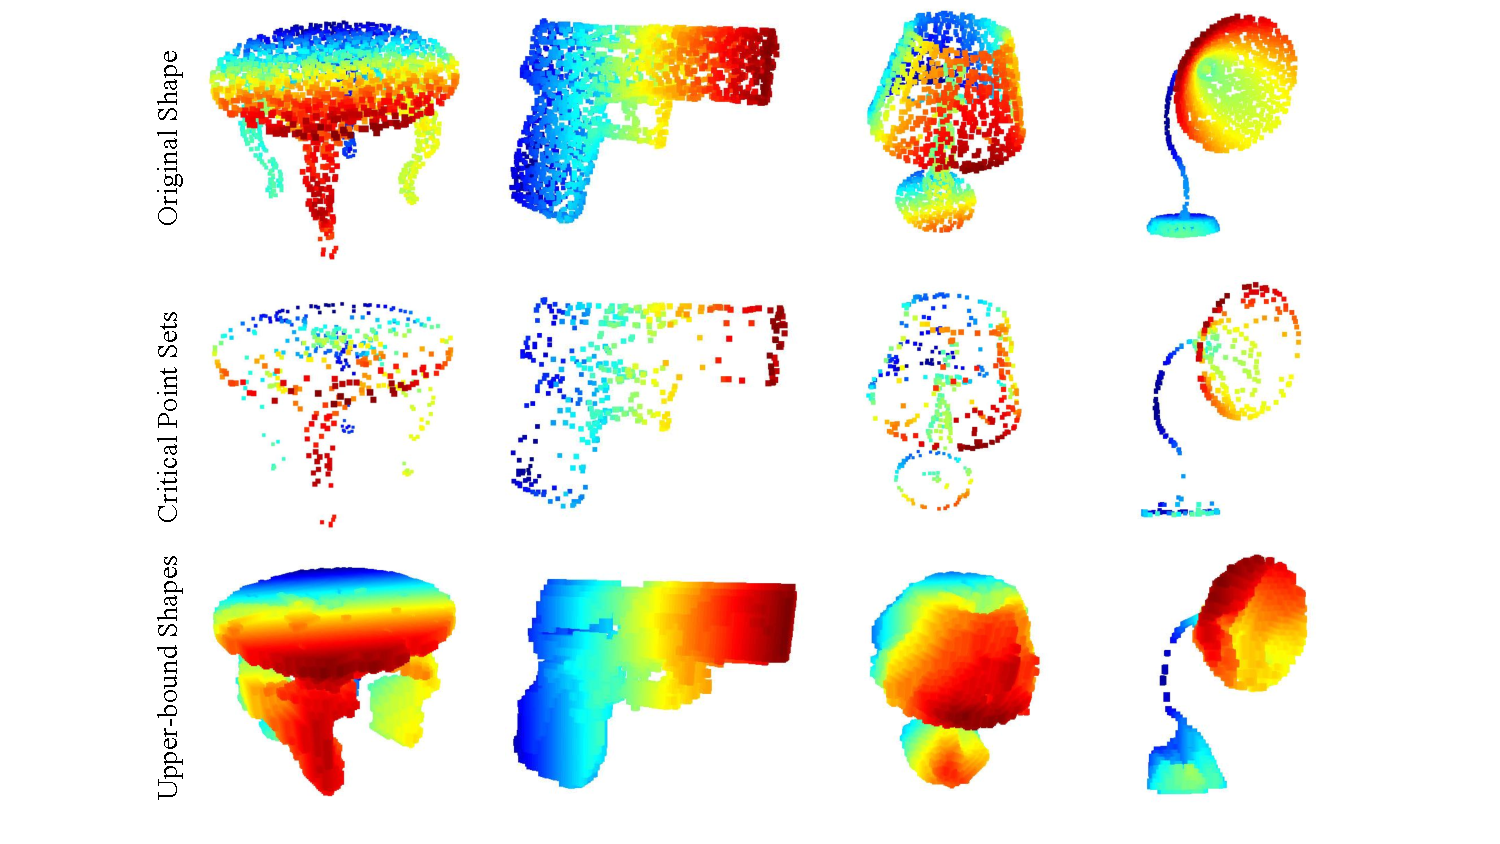
\includegraphics[width=0.9\linewidth]{fig/kp_ss_visu1.pdf}
% \caption{\textbf{Visualization of critical point sets and upper-bound shapes.} The first row shows the input point clouds $S$. The second and the third rows show the \textit{critical point sets} $\mathcal{C}_S$ and the \textit{upper-bound shapes} $\mathcal{N}_S$ respectively.}
% \label{fig:kp_ss_visu}
% \end{figure*}